\section{Theory of Algebraic Number}
\subsection{Norm, Trace and Discriminant}

For any finite extension \(L/K\) of degree \(n\), we can view element \(a \in L\) as a \(K\)-linear map
\[m_a: L \to L, \quad x \mapsto ax\]
in pariticular, it is an automorphism of \(L\) if \(a \neq 0\), and it satifies several properties:
\begin{itemize}
  \item \(m_{a+b} = m_a + m_b\)
  \item \(m_{ab} = m_a \circ m_b\)
  \item \(m_{c\cdot a} = c\cdot m_a\)
\end{itemize}
with \(a,b \in L\) and \(c \in K\). Since \(L\) is a finite-dimensional, it is natural to consider \(m_a\) as a matrix and define two invariants in linear algebra\\

- Trace of \(a\) over \(K\): \(\mathrm{Tr}_{L/K}(a) = \mathrm{Tr}(m_a)\)\\

- Norm of \(a\) over \(K\): \(\mathrm{N}_{L/K}(a) = \det(m_a)\)\\

exactly what we do can be concluded as the following
\[L \hookrightarrow \End_K(L) \to K\]
the first map refers to a \textbf{regular representation} of \(L\) over \(K\), and the second map is what we are familar with, and we can verify some properties of trace and norm:
\begin{itemize}
  \item \(\mathrm{Tr}_{L/K}(a+b) = \mathrm{Tr}_{L/K}(a) + \mathrm{Tr}_{L/K}(b)\)
  \item \(\mathrm{Tr}_{L/K}(c\cdot a) = c\cdot \mathrm{Tr}_{L/K}(a)\)
  \item \(\mathrm{N}_{L/K}(ab) = \mathrm{N}_{L/K}(a)\cdot\mathrm{N}_{L/K}(b)\)
  \item \(\mathrm{N}_{L/K}(c\cdot a) = c^n \cdot \mathrm{N}_{L/K}(a)\)
  \item \(\mathrm{Tr}_{L/K}(c) = nc\) and \(\mathrm{N}_{L/K}(c) = c^n\)
\end{itemize}
with \(a,b \in L\) and \(c \in K\). We can also give a more explicit description of trace and norm by the minimal polynoimal of \(a\) over \(K\), moreover, for any endomorphism \(m_a\) we can consider its \textbf{characteristic polynomial} \(\chi_a(t) = \det(t\cdot \mathrm{id}_L - m_a)\), and conclude the following result:

\begin{colorproposition}
  For any \(L/K\) finite extension with degree \(n\) and \(a \in L\),
  \begin{enumerate}[(a)]
    \item \(\chi_a = (\Pi_a)^d\) with \(d = [L:K(a)]\).
    \item Suppose \(\Pi_a(t) = t^m + c_{m-1}t^{m-1}+...+c_0\), then \[\mathrm{Tr}_{L/K}(a) = -dc_{m-1} \qquad \mathrm{N}_{L/K}(a) = (-1)^{n}c_0^d\]
  \end{enumerate}
\end{colorproposition}

\begin{proof}
  (a) It is clear that \(\deg \Pi_a = [K(a):K]\), we denote it by \(m\), then 
  \[\Pi_a(t)\ = t^m + c_{m-1}t^{m-1}+...+c_0\]
  for some \(c_i \in K\), and \(\{1,a,...,a^{m-1}\}\) is a basis for \(K(a)/K\), we suppose that \(\{e_1,..,e_d\}\) is a basis for \(L/K(a)\), then we can conclude a basis of \(L/K\) is
  \[e_1,\dots,e_1a^{m-1} \mid e_2,\dots,e_2a^{m-1} \mid \dots \mid e_{d},\dots,e_da^{m-1}\]
  so we can write the matrix of \(m_a\) under this basis
  
  \[m_a \sim \mathrm{diag}(A_1,\dots,A_d), \quad A_i = \begin{pmatrix}
    0 & 0 & \dots & -c_0 \\
    1 & 0 & \dots & -c_1 \\
    0 & 1 & \dots & -c_2 \\
    \vdots & \vdots & \ddots & \vdots \\
    0 & 0 & \dots & -c_{m-1}
  \end{pmatrix}\]
  By caclulate the characteristic polynomial of \(A_i\) we can get exactly
  \[\chi_a(t) = \prod_{i = 1}^d \det(t\cdot I- A_i) = (\Pi_a(t))^d\]
  (b) By vieta's formula we can conclude that
  \[\chi_a(t) = t^{n} - \mathrm{Tr}_{L/K}(a)t^{n-1} + \cdots + (-1)^n\mathrm{N}_{L/K}(a)\]
  then by formula of (a) we can caclculate the result.
\end{proof}

The invariant behaves well in separable extension (especially, Galois extension), for example the number fields, the reason is that we can talk about the conjugations of elements with invariant.

\begin{colorproposition} \label{tracenormformule}
  Let \(L/K\) be a separable finite extension of degree \(n\), then \\

  - \(\mathrm{N}_{L/K}(a) = \prod_{\sigma} \sigma(a)\) \\

  - \(\mathrm{Tr}_{L/K}(a) = \sum_{\sigma} \sigma(a)\)\\

  - \(\chi_a(X) = \prod_{\sigma} (X - \sigma(a))\)\\
  where \(a \in L\) and \(\sigma \in \Hom_K(L,\bar{K})\) runs over all \(K\)-embeddings
\end{colorproposition}

\begin{proof}
  We consider a relation of equivalence for \(\Sigma = \Hom_{K}(L,\bar{K})\) by
  \[\sigma_1 \sim_a \sigma_2 \iff \sigma_1(a) = \sigma_2(a)\]
  it holds for any finite extension, then we calculate the class of equivalence:
  \begin{align*}
    [\sigma] &= \{\tau \in \Sigma \mid \tau(a) = \sigma(a)\} \\
    &= \{\tau \in \Sigma \mid \tau(p(a)) = \sigma(p(a)) , \forall p \in K[X]\}\\
    &= \{\tau \in \Sigma \mid \tau = \sigma \text{ on } K(a)\}
  \end{align*}
  which shows that \( |[\sigma]| = |\Hom_{K(a)}(L,\bar{K})|\), in particular, if \(L/K\) is separable, then \(L/K(a)\) is also separble, so exactly \(|[\sigma]| = [L:K(a)]\), it implies
  \[\prod_{\sigma}(X-\sigma(a)) = \prod_{[\sigma] \in \Sigma/\sim_a} (X-\sigma(a))^{[L:K(a)]} = \Pi_a(X)^{[L:K(a)]} = \chi_a(X)\]
  Here \(\sigma(a)\) runs over all roots of \(\Pi_a\) since the restriction map
\[res: \Hom_K(L,\bar{K}) \to \Hom_K(K(a),\bar{K}), \quad \sigma \mapsto \sigma|_{K(a)}\]
is srujective.

\end{proof}

\begin{definition}
  Let \(L/K\) be a finite extension of degree \(n\)\\
  - The \textbf{trace pairing} of the extension is a symmetric \(K\)-bilinear form
  \[Q_{L/K}(x,y) =  \mathrm{Tr}_{L/K}(xy)\]
  - we define the \textbf{discriminant} of a family \(\{e_1,\dots,e_n\}\) in \(L\)  by
\[\mathrm{Disc}(e_1,...,e_n) = \det(\mathrm{Tr}_{L/K}(e_ie_j)) = \det(Q_{L/K}(e_i,e_j)) \]
\end{definition}

It is better to consider the discriminant in a separable extension, although we always use the \textbf{"free condition"} in the extension of \(\qq\), the reason is as following:

\begin{proposition}
  Let \(L/K\) be a finite extension, then the following conditions are equivalent:
  \begin{enumerate}
    \item \(L/K\) is separable.
    \item \(\mathrm{Tr}_{L/K} \neq 0\).
    \item The trace pairing \(Q_{L/K}\) is non-degenerate.
  \end{enumerate}

\end{proposition}

\begin{proof}
  
\end{proof}

\begin{remark}
  Consider the inseparable example of \(L = \ff_p(t^{1/p})\), we can calculate  \(\mathrm{Tr}_{L/K}(u^k) = 0\) with \(u = t^{1/p}\) and \(k = 0,1,...,p-1\), which shows that the trace is identically zero, so the discriminant of any basis is zero, which provides no information about the extension.
\end{remark}

\begin{colorproposition}
  Let \(L/K\) be a finite separable extension of degree \(n\), and \(a_1,...,a_n\) be a basis of \(L/K\), then the discriminant of the basis 
  \[\mathrm{Disc}(a_1,...,a_n) = \det(\mathrm{Tr}_{L/K}(\sigma_i(a_j)))^2\]
  with \(\sigma_i \in \Hom_K(L,\bar{K})\) \(n\) distinct \(K\)-embeddings of \(L\). 
\end{colorproposition}

\begin{proof}
  Review that for any two n order square matrices \(A,B\), we have
  \[(AB)_{i,j} = \sum_{k=1}^n A_{i,k} B_{k,j}\]
  In particular
  \[(A^TA)_{i,j} = \sum_{k=1}^n A_{k,i}A_{k,j}\]
  so For any \((i,j)\)-entry of trace matrix, applying proposition \ref{tracenormformule} we can calculate
  \[\mathrm{Tr}_{L/K}(a_ia_j) = \sum_{k=1}^n \sigma_k(a_i)\sigma_k(a_j) = 
  \sum_{k=1}^n \sigma_k(a_i)\sigma_k(a_j) = \sum_{k=1}^n = (A^TA)_{i,j}\]
  where \(A = \mathrm{Tr}_{L/K}(\sigma_i(a_j))_{1 \leq i,j \leq n}\).
\end{proof}

\begin{colorcorollary}
  Let \(L/K\) be a finite separable extension of degree \(n\), then the discriminant of any basis of \(L/K\) is no-zero, in particular, if \(a\) is the primitive element such that \(L=K(a)\) and \(\{1,...,a^{n-1}\}\), then
  \[\Disc(1,a,...,a^{n-1}) = \prod_{i<j}(r_i-r_j)^2\]
  where \(r_i\) are the distinct \(n\) roots of \(\Pi_a\) in \(\bar{K}\).
\end{colorcorollary}

\begin{proof}
  Review that 
  \[(PAP^T)_{i,j}  = \sum_{1\leq k,l \leq n}P_{i,k}P_{j,l}A_{k,l}\]
  For any two n order square matrices \(A,P\).
  For any basis \(\{e_1,...,e_n\}\), there exists a invertible matrix \(P\) such that \(e_i = \sum_{j=1}^n P_{ij} a^{j-1}\), since \(\{1,\dots,a^{n-1}\}\) is a basis, then 
  \begin{align*}
    \mathrm{Tr}_{L/K}(e_ie_j) &= \mathrm{Tr}_{L/K}\left(\left(\sum_{k=1}^n P_{ik} a^{k-1}\right)\left(\sum_{l=1}^n P_{jl} a^{l-1}\right)\right) \\
    &= \sum_{k,l=1}^n P_{ik}P_{jl}\mathrm{Tr}_{L/K}(a^{k+l-2}) \\
    &= \sum_{k,l=1}^n P_{ik}P_{jl}\mathrm{Tr}_{L/K}(a^{k+l-2})
  \end{align*}
  which shows that the trace matrix of the basis is \(P^T A P\), where \(A = (\mathrm{Tr}_{L/K}(a^{i-1}a^{j-1}))_{i,j}\), which suffice to calculate that
  \[\Disc(e_1,...,e_n) = |\det(P)|^2 \Disc(1,a,\dots,a^{n-1}) \]
  Hence just need to calculate the discriminant of the basis \(\{1,...,a^{n-1}\}\), and prove that it is non-zero, which finishes the proof. By the above proposition, we can calculate
  \[\Disc(1,a,\dots,a^{n-1}) = \begin{vmatrix}
    1 & \sigma_1(a) & \dots & \sigma_1(a)^{n-1} \\
    1 & \sigma_2(a) & \dots & \sigma_2(a)^{n-1} \\
    \vdots & \vdots & \ddots & \vdots \\ 
    1 & \sigma_n(a) & \dots & \sigma_n(a)^{n-1}
  \end{vmatrix}^2\]
  where \(\sigma_i(a)\) runs over all distinct roots since \(L/K\) is separable, hence we can conclude the result by the \textbf{Vandermonde determinant formula}.

  \begin{remark}
    \textbf{A remakrable fact} in the proof is the scale of the discrimniant, suppose that \(\{e_1,\dots,e_n\}\) and \(\{a_1,\dots,a_n\}\) are two family with \([e_1,\dots,e_n] = P[a_1,\dots,a_n]\) for some endomorphiosm \(P\), then 
    \[\mathrm{Disc}(e_1,\dots,e_n) = |\det(P)|^2 \mathrm{Disc}(a_1,\dots,a_n)\]
  \end{remark}

\end{proof}
\subsection{Number fields}

To motivate the algebraic approach, we firstly consider a typical example in number theory, it will be the basis of the discussion.

\begin{itemize}
    \item The finite extension of \(K/\qq\) is called a \textbf{number field}, typically it an separable extension since \(\mathrm{Char}(\qq) = 0\), so we can apply \textbf{primitive element} theorem to conclude that \(K = \qq(a)\) for some \(a \in K\).
    \item The element \(a \in K\) is called an \textbf{algebraic integer} if there exists a monic polynomial \(f(x) \in \zz[x]\) such that \(f(a) = 0\). Notice that the following conditions are equivalent:
    \begin{enumerate} [(a)]
        \item \(a\) is an algebraic integer.
        \item minimal polynomial \(\Pi_a(X) \in \zz[X]\).
        \item \(\zz[a]\) is a finitely generated \(\zz\)-module.
    \end{enumerate}
    \begin{proof}
        
    \end{proof}

    \item Following the above definition, we can verify a similar result with the algebraic numbers: (a) sum of two algebraic integers is an algebraic integer, (b) product of two algebraic integers is an algebraic integer.
    \begin{proof}
        
    \end{proof}
    \item It is trival that algebraic integers are algebraic numbers, so similarly we can define
    \[\tilde{\qq} = \{x \in \bar{\qq} : x \text{ is an algebraic integer}\}\]
    It is a subring of algebraic closed field \(\bar{\qq}\) or \(\cc\), and then we can define the ring of integers of number field \(K\) as 
    \[\ok := \tilde{\qq} \cap K\]
    equivalently, it is the set of all algebraic integers contained in \(K\). 
\end{itemize}

So we skecth the basic notation and definitions, the ring of integers of number field is special and important, since it is analogous to \(\zz\) in \(\qq\), and in particualr number theory is the study of "integers", although here the integraility is not clear, so we will focus on it.

\begin{colortheorem}
    Let \(K/ \qq\) be a number field with \(\ok\) its ring of intgers, then
    \begin{enumerate}
        \item \((\ok,+)\) is a free \(\zz\)-module of rank \([K:\qq]\), hence it is a noetherian ring.
        \item \(\ok\) is integrally closed in \(K\) (following the definition).
        \item Any non-zero prime ideal in \(\ok\) is maximal, i.e. the krull dimension of \(\ok\) is 1.
    \end{enumerate}
\end{colortheorem}
\begin{proof}

\end{proof}

To study the arithmetic of "integers" we should understand the factorization of elements in \(\ok\), unfortunately, the ring of integers are not always UFD, typcial example is \(\ok = \zz[\sqrt{-5}]\) with \(K = \qq(\sqrt{-5})\), in it we have
\[6 = 2 \times 3 = (1 + \sqrt{-5})\times (1 - \sqrt{-5})\]
even more terrible, for the simplest example \(K=\qq(\sqrt{d})\) ( \(d\) is square-free), we have the following known results:\\

- When \(d<0\), \(\ok\) is a UFD if and only if \(d\) is one of the following integer:
\[-1,-2,-3,-7,-11,-19,-43,-67,-163\]
It is owe to the \textbf{Heegner-Baker-Stark theorem}, and the proof is non-trivial.\\

- When \(d>0\), it is conjectured by Gauss that there are infinitely many \(d\) such that \(\ok\) is a UFD, but it is still open (till 2026...).\\

Hence it is almost hopeless to consider the factorization of elements in \(\ok\). After dedekind and Kummer introduced the concept of ideal, a more general factorization is possible, in particular it holds for any number fields.

\begin{colortheorem} \label{fract}
    For any number field \(K\) with ring of integers \(\ok\), any non-zero proper ideal \(I \subsetneq \ok\) can be factored into prime ideals, i.e. there exist prime ideals \(\pp_1,\cdots,\pp_n\) such that
    \[I = \pp_1 \cdots \pp_n\]
and the factorization is unique up to permutation of the prime ideals.
\end{colortheorem}

For example we consider \(\ok = \zz[\sqrt{-5}]\), we have the following factorization of ideals:
\[(6) = \mathfrak{p}_2^2 \mathfrak{p}_3 \mathfrak{p}_3'\]
with \[\mathfrak{p_2} = (2,1+\sqrt{-5}),\quad \mathfrak{p_3} = (3,1+\sqrt{-5}),\quad \mathfrak{p_3'} = (3,1-\sqrt{-5})\]
then we can find that the factorization of \(6\) is unique in the sense of ideals:
\[(2) = \mathfrak{p}_2^2 , \quad (3) = \mathfrak{p}_3 \mathfrak{p}_3'\]
while
\[(1+\sqrt{-5}) = \mathfrak{p}_2 \mathfrak{p}_3 ,\quad (1-\sqrt{-5}) = \mathfrak{p}_2 \mathfrak{p}_3'\]

To prove the theorem, some preparation should be done since the result is eseentailly not trival, firstly we should consider the division of ideals:

\begin{definition}
    Let \(\mathfrak{a}\) and \(\mathfrak{b}\) be two non-zero ideals in \(\ok\), we define 
    \[\mathfrak{a} | \mathfrak{b} \iff \mathfrak{b} \subset \mathfrak{a}\]
\end{definition}

This definition can be done for any commutative ring, but the properties of rings of integers ensures the following results, which is the key to the proof.

\begin{lemma}
    \(\pp\) is a prime ideal of \(\ok\) if and only if for any ideals \(\mathfrak{a}\) and \(\mathfrak{b}\) in \(\ok\), we have \(\pp | \mathfrak{a}\mathfrak{b} \implies \pp | \mathfrak{a} \text{ or } \pp | \mathfrak{b}\).
\end{lemma}
\begin{proof}
    
\end{proof}

\begin{lemma}
    For any non-zero ideals \(\mathfrak{a} \in \ok\), there exists non-zero prime ideals \(\mathfrak{p_1},\cdots,\mathfrak{p_n}\) such that \( \mathfrak{p_1}\cdots\mathfrak{p_n} \subset \mathfrak{a}\). 
\end{lemma}

\begin{proof}
    
\end{proof}

\begin{lemma} \label{lemma2forfract}
    For any prime ideal \(\pp\) in \(\ok\), we define its inverse ideal as \[\pp^{-1} = \{x \in K : x\pp \subset \ok\}\]
then for any non-zero ideal \(\mathfrak{a}\) in \(\ok\), we have \(\mathfrak{a}\subsetneq \mathfrak{a}\pp^{-1} \). In particular, \(\pp\pp^{-1} = \ok\).
\end{lemma}
\begin{proof}
    
\end{proof}

With the two lemma we can finish the proof:
\begin{proof}[Proof of theorem \ref{fract}]
    For the existence, we set a set \(S\) of ideals which can not be factorized into prime ideals, if \(S\) is empty then we are done, \textbf{hence we assume \(S\) is non-empty}. We consider the partial ordered set \((S,\subset)\), then the noetherian condition ensures the existence of maximal element, denoted by \(\mathfrak{a}\).

    \(\mathfrak{a}\) can not be prime (i.e. maximal), otherwise it is already factorized, hence there exists a maxiaml ideal (i.e prime) such that \(\mathfrak{a} \subsetneq \pp\), which implies
    \[\mathfrak{a} \subsetneq \mathfrak{a}\pp^{-1} \subsetneq \pp\pp^{-1} = \ok \]
    the chain holds trus by lemma \ref{lemma2forfract}, hence we construct an element \(\mathfrak{a}\pp^{-1} \notin S\), which allows us to factorize
    \[\mathfrak{a}\pp^{-1} = \pp_1 \cdots \pp_r\]
    then \(\mathfrak{a} = \mathfrak{a}\ok = \mathfrak{a}\pp^{-1}\pp\) shows that the maximal element can be factorized, which is a contradiction.

    For the uniqueness, we assume that there are two factorization for an ideal \(\mathfrak{a}\)
    \[\mathfrak{a} = \mathfrak{p}_1\cdots \mathfrak{p}_n = \mathfrak{q}_1 \cdots \mathfrak{q}_m\] 
    then \(\pp_1 | \mathfrak{a}\) shows that there exists \(i\) such that \(\pp_1 | \mathfrak{q}_i\), prime ideals are maximal so \(\pp_1 = \mathfrak{q}_i\) exactly, and we can cancel then by multiplying \(\pp^{-1}\), then we can repeat the process to conclude that \(n=m\) and \(\pp_i = \mathfrak{q}_{\sigma(i)}\) for any permutation \(\sigma \in S_n\).
\end{proof}

with unique factorization, we can extend the definition of norm from elements to ideals.

\begin{colordefinition}
    For any non-zero ideal \(\mathfrak{a}\) in \(\ok\), we define its \textbf{(aboslute) norm} by
    \[N(\mathfrak{a}) = |\ok / \mathfrak{a}|\]
    where \(\ok/\mathfrak{a}\) is called the \textbf{residue ring} of \(\mathfrak{a}\). 
\end{colordefinition}

\begin{remark}
    The definition should be clarified, any non-zero ideal \(\mathfrak{a}\) is exactly a \(\zz\)-submodule of \(\ok\), while \(\ok\) is free and \(\zz\) is PID, hence \(\mathfrak{a}\) is a free \(\zz\)-module with rank \(\leq n = [K:\qq]\). We can take any non-zero element \(x\) of \(\mathfrak{a}\) such that we have a chain 
    \[(x) \subset \mathfrak{a} \subset \ok\]
    principal ideal must be a free \(\zz\)-module of rank \(n\) by an \(\zz\)-module isomorphism with \(\ok\), hence the chain forces \(\mathfrak{a}\) is also a free \(\zz\)-module of rank \(n\), hence the residue ring is exactly finite.
\end{remark}

\begin{colorproposition}
    Let \(K\) be a number field with ring of integers \(\ok\)
    \begin{enumerate} [(a)]
        \item For non-zero ideals \(\mathfrak{a}\) with fractorization \(\mathfrak{a} = \pp_1^{r_1} \cdots \pp_n^{r_n}\)
        \[N(\mathfrak{a}) = N(\mathfrak{p}_1)^{r_1} \cdots N(\mathfrak{p}_n)^{r_n}\]
        \item Norm is \textbf{multiplicative}, i.e. \(N(\mathfrak{ab}) = N(\mathfrak{a})N(\mathfrak{b})\) for any two non-zero ideals.
        \item Let \(\mathfrak{a}\) be a non-zero ideal with \(\zz\)-basis \(\{a_1,\cdots,a_n\}\), then
        \[N(\mathfrak{a})= \sqrt{\frac{d_{a}}{d_K}}\]
        \item For principal ideal, \(N((a)) = |N_{K/\qq}(a)|\) with \(a \) non-zero in \(\ok\).
    \end{enumerate}
\end{colorproposition}
\begin{proof}
    If the factorization of a non-zero ideal \(\mathfrak{a}\) is \(\mathfrak{a} = \pp_1^{r_1} \cdots \pp_n^{r_n}\), then by Chinese remainder theorem, the residue ring can be decomposed as
\[\ok/\mathfrak{a} \cong \ok/\mathfrak{p_1}^{r_1} \times \cdots \times \ok/\mathfrak{p_n}^{r_n}\]
hence it is enough to prove that for any prime ideal \(\pp\) we have \(N(\mathfrak{p}^k) = N(\mathfrak{p})^k\). For any \(i \geq 1\), \(\mathfrak{p}^i/\mathfrak{p}^{i+1}\) is a \(\ok/\mathfrak{p}\)-vector space since \(\mathfrak{p}\) is a \(\ok\)-module,
\[\mathfrak{p}^i/\mathfrak{p}^{i+1}\cong \ok/\mathfrak{p}\otimes_{\ok} \mathfrak{p}^i \]
consider \(k = \ok/\mathfrak{p}\), then \(k\) is the residue field of local ring \(\mathcal{O}_{K,\mathfrak{p}}\), hence 
\begin{align*}
    \mathfrak{p}^i/\mathfrak{p}^{i+1} &\cong (k \otimes_{\ok} \mathcal{O}_{K,\mathfrak{p}}) \otimes_{\ok} \mathfrak{p}^i \\
    &\cong k \otimes_{\mathcal{O}_{K,\mathfrak{p}}} \mathfrak{p}^i \mathcal{O}_{K,\mathfrak{p}} \\
    &\cong k
\end{align*}
which shows that \(\mathfrak{p}^i/\mathfrak{p}^{i+1}\) is one-diemnsional over \(k\) \textbf{(an alternative proof can be found in \cite{Tall} Lemma 6.20 , with direct discussion isomorphism)}, hence we can conclude that
\[N(\mathfrak{p}^k) = |\ok/\mathfrak{p}|\cdot|\mathfrak{p}/\mathfrak{p}^2|\cdots |\mathfrak{p}^{k-1}/\mathfrak{p}^k| = N(\mathfrak{p})^k\]
which finishes the proof of (a), and (b) is a direct consequence of (a).

For (c), 
\end{proof}


\textcolor{blue}{Similarly with Gauss integer, the norm of an ideal can be used to determine whether it is prime, and it will open a complicated story about the arithemtic of number fields.}

\begin{lemma}
    Let \(\mathfrak{p}\) be a non-zero prime ideal of \(\ok\), then
    \begin{enumerate} [(a)]
        \item there exists a unique prime number \(p\) such that \(p \in \mathfrak{p}\).
        \item \(N(\pp) = p^e\) for some integer \(1\leq e \leq n\).
        \item \(\pp \cap \zz = (p)\).

    \end{enumerate}
\end{lemma}

\begin{proof}
    Notice \(\mathcal{O}_k/\pp\) is a finite field if \(\pp\) is prime (in \(\ok\) it is maxiaml), which proves (b). For (c), notice that \(\pp \cap \zz\) is pre-image of \(\pp\) under the inclusion \(\zz \hookrightarrow \ok\), and the contraction of a prime ideal is either zero or a prime ideal. \(\pp \cap \zz\) can't be zero, in fact we take any non-zero \(x \in \pp \subset \ok\), then using the minimal polynomial \(\Pi_x \in \zz[X]\), we can deduce that \(f = \Pi_x-\Pi_x(0) \in \zz[X]\) is a polynomial such that \(f(x) = -\Pi_x(0) \in \zz\), which shows that\(f(x) \in \pp \cap \zz\), and it proves (b). For (a), (c) shows the existsence of prime number \(p\) exactly, if there are another prime number \(q \in \pp\) then
    \[N(\mathfrak{p}) \text{ divise } N(p)=p^n, \quad N(\mathfrak{p}) \text{ divise } N(q)=q^n \]
    it show taht \(N(\pp) = 1\), it is impossible.
\end{proof}

The properties of prime ideals invite some vocabulary, for any prime number \(p\), there exists a factorization in sense of principla ideal
\[(p) = \pp_1^{e_1} \cdots \pp_k^{e_k}\]

a prime ideal \(\pp\) is called \textbf{lying over \(p\)} if \(\pp | (p)\), and the \textbf{ramification index} of \(\pp\) is defined as 
    \[e  = \max \{l \in \nn : \pp^l | (p) \}\]
and the \textbf{residue index} of \(\pp\) is defined as the extension degree
\[f = [\ok/\pp : \ff_p]\]
    exactly such \(\pp\) must be one of \(\pp_i\) with \(e_i\) as its ramification index, and residue index is just the expoent \(f_i\) such that \(N(\pp_i) = p^{f_i}\), hence we immediately we have the following relation

\begin{colorcorollary}
    \[[K:\qq] = \sum_{\pp_i} e_if_i \]
    where \(\pp_i\) runs over all prime ideals lying over \(p\), with \(e_i\) and \(f_i\) as its ramification index and residue index respectively.
\end{colorcorollary}

We can talk more about the factorization of prime numbers, which is the basis of the study of arithemtic of number fields.

\begin{enumerate}
    \item For any number field \(K\), as a separable extension there eixsts \(a \in K\) such that \(K = \qq(a)\) and \(\ok = \zz[a] \cong \zz[X]/(\Pi_a(X))\). We want to study \((p) = p\ok\) for some \textbf{integral prime} \(p\), so it is natural to consider the quotient \(\ok/p\ok\): if the quoitent is a field or just integral domain, we can determine that \((p)\) is prime.

    \item Otherwise, we consider \(\ok\) as a \(\zz\)-module
    \[\ok/p\ok \cong (\zz/(p)) \otimes_{\zz} \zz[X]/(\Pi_a) \cong \ff_p[X]/(\overline{\Pi}_a)\]
    we consider the factorization of \(\bar{\Pi}_a\) in \(\ff_p[X]\), it will be unique since \(\ff_p[X]\) is a PID, so by chinese remainder theorem we can decompose the quotient as a product 
    \[\ok/p\ok \cong \prod_{i}\ff_p[X]/(\bar{Q}_i^{e_{i}})\]
    notice that the structure is analogoue to the factorization of ideals \((p) = \prod_i \pp^{e_i}\), so it is natural to find \(\pp_i\) by consider the lifting of each irreducible factor \(\bar{Q}_i\), so it motivates us to define
    \[I_p(Q) = p\ok + Q(a)\ok\]
    where \(Q \in \zz[X]\) is a monic polynomial such that \(\bar{Q} \in \ff_p[X]\) is a factor of \(\bar{\Pi}_a\).

    \item Notice that \(\bar{a} \mapsto \bar{X}\) gives the first isomorphism in 2, so if \(\bar{Q}\) is a irreducible factor of \(\bar{\Pi}_a\), then  we can conclude  \[I_p(Q)/p\ok \cong (Q)/(Q^{e})\] this is the maximal ideal in local ring \(\ff_p[X]/(Q^{e})\), so by this isomorphism we can conclude that \textbf{\(I_p(Q)\) is the maximal (so prime) ideal.}
    
    \item The lifting \(Q\) is not unique, but \(I_p(Q)\) \textbf{does not depend on the choice of} \(Q\): In fact if we set \(Q' \in \zz[X]\) as another lifting of \(\bar{Q}\), then \(Q(a) - Q'(a) = 0 \mod p\), which shows that \(Q(a) \in I_p(Q')\) and \(Q' \in I_p(Q)\) respectively, hence \(I_p(Q) = I_p(Q')\).
    
    \item In fact as we have known, the factorization of \((p)\) is unique, so in priori we can write the isomorphism \(\ok/p\ok \cong \prod_{i} \ok/\pp_i^{e_i}\), and \(I_p(Q)\) as we have shown is a prime ideal lying over \(p\), so we can conclude directly the following result (It is another view to prove the uniqueness of factorization of ideals)
\end{enumerate}


\begin{colortheorem}[Dedkind-Kummer] $\\$
    Let \(K\) be a number field with primitive element \(a\), and \(p \in \zz\) a prime, then
    \begin{enumerate} [(a)]
        \item The bijection \(Q \mapsto I_p(Q)\) gives a correspondence
        \[\{\text{monic factors of } \overline{\Pi}_a \in \ff_p[X]\} \leftrightarrow \{\text{ideal dividing } (p)\}\]
        \[\{\text{ irreducible factors}\} \leftrightarrow \{\text{prime ideals}\}\]
        \item The norm of \(I_p(Q)\) is \(p^{\deg(Q)}\). When \(\bar{Q}\) is a irreducible factor, \(\deg (Q)\) is exactly the residue index of \(I_p(Q)\).
        \item there exists integer \(e_i \in \nn\) such that
        \[(p) = \prod_i I_p(Q_i)^{e_i}\]
        where \(\bar{Q}_i\) runs over all distinct irreducible factors of \(\bar{\Pi}_a\) in \(\ff_p[X]\), and \(e_i\) is the multiplicity of \(\bar{Q}_i\) in \(\bar{\Pi}_a\), it is exactly the ramification index of \(I_p(Q_i)\).
    \end{enumerate}
    
\end{colortheorem}









\subsection{Minkowski's space}

This theory corresponds to the geometry of numbers, the idea is to consider embedding of number fields into \(\rr\) or \(\cc\), we now consider a number field \(K\) of degree \(n\), and review some basic notations:
    \begin{enumerate}
        \item an embedding \(\sigma: K \to \cc\) is called a \textbf{real embedding} if \(\sigma(K) \subset \rr\), otherwise it is called a \textbf{complex embedding}. Since \(K/\qq\) is separable, hence the number of embeddings is exactly \(n\).
        \item It is easy to verify that if \(\sigma\) is an embedding, then \(\bar{\sigma}\) is also an embedding, we say that two complex embeddings \(\sigma\) and \(\sigma'\) are conjugate if
        \(\sigma' = \bar{\sigma}\). Hence the set of embeddings can be divided as following:
        \[\Sigma = \Sigma_r \sqcup \Sigma_c \sqcup \bar{\Sigma}_c\]
        where \(\Sigma_r\) is the set of real embeddings, and \(\Sigma_c\) is the set of distinct complex embeddings up to conjugation. In particular, we set 
        \[\Sigma_0 = \Sigma_r \sqcup \Sigma_c \cong \Sigma / \sim\]
        to denote the set of distinct embeddings up to conjugation, and usually we write \(n = r+2s\) with
        \[r=|\Sigma_r|, \quad s = |\Sigma_c|\]
        3. For any \(\rr\)-vector space \(V\) of dimension \(n\) with an inner product \(\langle -,- \rangle\), an additive subgroup \(L \subset V\) is \textbf{a complete lattice} if \(V/L\) is compact (or equivalently, \(L\) is discrete of rank \(n\)), and we can define the volume and covlume
        \[\mathrm{covol}(L) = \mathrm{Vol}(V/L) = \mu(F)\]
        where \(\mu\) is the induced measure, and \(F\) is the fundamental domain. If \(L = \oplus_{i=1}^n \zz v_i\) for some basis \(\{v_1, \ldots, v_n\}\), then we have 
        \[\mathrm{covol}(L) =\mathrm{Vol}(V/L) = \sqrt{\det G}\]
        where \(G\) is the Gram matrix with entries \(G_{ij} = \langle v_i, v_j \rangle\).
    \end{enumerate}

    \begin{definition}
        For any number field \(K\) of degree \(n=r+2s\), we define the \textbf{Minkowski's space} of \(K\) as a \(\rr\)-vector space \(K_{\infty} = \rr^n\) together with an inner product defined by
        \[\langle x,y \rangle_m = \sum_{i=1}^n a_i \cdot x_iy_i\]
        with \[a_i = \begin{cases}
            1 \quad &\text{if } i \leq r\\
            2 \quad &\text{if } i > r
        \end{cases}\]
    \end{definition}

    \begin{remark}
        The Minkowski's space always appears together with the embedding of \(K\) by 
        \[\iota : K \hookrightarrow \rr^r\times \cc^s \cong K_{\infty} , \quad  x \mapsto (x_{\sigma})_{\sigma \in \Sigma_0} \]
        where \(x_{\sigma} = \sigma(x)\), the inner product can be pulled back to \(K\) by 
        \[\langle x,y \rangle_M = \langle \iota(x),\iota(y) \rangle_m = \sum_{\sigma \in \Sigma_0} a_\sigma \cdot \mathrm{Re}(x_\sigma \overline{y_\sigma})\]
        with  \[ a_\sigma = 
        \begin{cases}
           1 \quad &\text{if } \sigma \text{ real }\\
           2 \quad &\text{if } \sigma \text{ complex }
        \end{cases} \]
        \textbf{It is not hard to verify that the inner product concides with the trace pairing if \(K\) is totally real (\(s =0 \)).}

    \end{remark}

    \begin{remark}
        We can view that this inner product is the restriction of the Hermitian inner product on \(\cc^n\), i.e. it is same with the pulled back from the embedding
        \[K \to \cc^n , \quad x \mapsto (x_{\sigma})_{\sigma \in \Sigma}\]
        the reason to consider the restriction is that \(\rr\)-vector space is exactly the place where the convex geometry works, and we always view ideal as a lattice in the Minkowski's space, such that we can talk about the volume and the density. 
    \end{remark}

    \begin{colortheorem}[The structure of Minkowski's space]$ \\$
         Along the notation above
         \begin{enumerate} [(a)]
            \item \(K_{\infty} \cong K \otimes_{\qq} \rr\).
            \item A subset of \(K_{\infty}\) is measurable if and only if it is lebesgue measuable, in particular we they are distict up to a constant
            \[\mathrm{Vol}(S) = 2^{s}\cdot \mathrm{Vol}_{Lebesgue}(S) \]
            \item If \(\mathfrak{a}\) is a non-zero ideal in \(\ok\), then \(\iota(\mathfrak{a})\) is a lattice in \(K_{\infty}\) with \[\mathrm{covol}(\iota(\mathfrak{a})) = \sqrt{|d_{\mathfrak{a}}|}\]
            Moreover, the aboslute norm of \(\mathfrak{a}\) can be defined \textbf{equivalently} by
            \[N(\mathfrak{a}) = \frac{\mathrm{covol}(\iota(\mathfrak{a}))}{\mathrm{covol}(\iota(\ok))}\]
         \end{enumerate}
        
    \end{colortheorem}
    \begin{proof}
        (a)

        (b) The inner product is the euclidean inner product with weight, hence the norm are equivalent to the standard norm. Notice that the lebesgue measure and induced measure on Minkowski's space are both Haar measure, so they are distinct up to a constant, so it is enough to compute the hypercube \(S = [0,1]^n\) in both measures, and we have
        \[\mathrm{Vol}(S) = \sqrt{\det (\langle e_i,e_j \rangle_m)_{i,j}} = 2^s \]
        (c) Review that for square matrix \(A\) we have 
        \[(A^T\bar{A})_{i,j} = \sum_{k} A_{k,i} \overline{A_{k,j}}\]
        by definition of the discriminant, if \(a_1,\dots,a_n\) is a basis of \(\mathfrak{a}\), then we have
        \[d_{\mathfrak{a}} = \det[\sigma_i(a_j)]^2\]
        hence we set here \(A\) is the matrix with entries \(A_{i,j} = \sigma_i(a_j)\), then we have
        \[(\bar{A}^TA)_{i,j} = \langle a_i, a_j \rangle_M\]
        hence \(\mathrm{covol}(\iota(\mathfrak{a})) = \sqrt{\det (\bar{A}^TA)}  = |\det A| = |d_{\mathfrak{a}}|\), notice here \(A \in M(n,\cc)\) exactly with \(\det A \in \cc\).

    \end{proof}

    \begin{remark}
        In sense of Minkowski's space, the discriminant of a number field \(K\) can be described as a geometric invariant, it is eaxctly the square of the volume of the fundamental domain with respect to the translation action \(\ok\) on \(K_{\infty}\).
    \end{remark}

    Since \(\iota\) is an inclusion, so we it has no problem to identify the subset of \(K\) (numbers) as the subset of \(K_{\infty}\) (vectors), from now on we will not distinguish them with a littble abusion of notation, i.e.
    \[  \mathrm{Vol}(S)  = \mathrm{Vol}(\iota(S)) \]
    for any subset \(S \subset K\) (or \(K_{\infty}\)).

    \begin{theorem}[Minkowski's convex theorem] $ \\$
        Let \(K\) be a number field of degree \(n\) with ring of integers \(\ok\), and let \(\iota(S) \subset K_{\infty}\) be a convex symmetric measurable subset with 
        \[\mu(\iota(S)) > 2^n \cdot \mu(\iota(\ok))\]for any Haar measure on \(K_{\infty}\), then there exists a non-zero element \(x \in \ok\) such that \(\iota(x) \in S\).
    \end{theorem}

    \textbf{The proof is owe to the theory of lattice, should pay attention to the habite that we usually consider the lebesgue measure \(\lambda\), and choose a proper convex body we can get some interesting results about number fields.}

    \begin{colortheorem}
        For any non-zero ideal \(\mathfrak{a}\) in \(\ok\), there exists a non-zero element \(a \in \mathfrak{a}\) such that
        \[|N_{K/\qq}(a)| \leq M_K N(\mathfrak{a})\]
        where \(M_k = \frac{n!}{n^n}(\frac{4}{\pi})^s\sqrt{|d_K|}\) is defined as the \textbf{Minkowski's bound} of \(K\).
    \end{colortheorem}

    \begin{proof}
        We define a \(L^1\) norm on \(K_{\infty}\) by
        \[\|(x_1,\dots,x_r,z_1,\dots,z_s)\|_1 = \sum_{i=1}^r |x_i| + 2\sum_{i=1}^s  |z_i|\]
        and then under this norm we define a convex symmetric body by
        \[C_R = \{x \in K_{\infty} : \|x\|_1 \leq R\}, \quad R>0\]
        then we can calculate the volume \(\lambda(C_R) = 2^r(\frac{\pi}{2})^s\frac{R^n}{n!} \), and then we apply Minkowski's theorem here to conclude the lower bound of \(R\) such that \(\mathfrak{a} \cap \iota^{-1}(C_R) \neq \emptyset\) will be
        \[R^n \geq n! \cdot \frac{2^{n-r}}{\pi^s} \cdot N(\mathfrak{a}) \sqrt{|d_K|}\]
        under this condition, we set \(a \in \mathfrak{a}\) to be a such element, to estimate the norm of \(a\), we apply \textbf{the inequality of arithmetic and geometric means} to get
        \begin{align*}
            |N_{K/\qq}(a)| &= \prod_{\sigma \in \Sigma} |\sigma(a)| \\
            &\leq \frac{1}{n^n} \|\iota(a)\|_1^n \\
            &\leq \frac{R^n}{n^n}
        \end{align*}
        so it is enough to take the lower bound
         of \(R\) to finishe the proof.
    \end{proof}

    \subsection{Logarithmic space and Unit theorem}
    This section is the complement of the the last section, and the notation will be the same as before for the sake of consistency. 

    \begin{definition}
        The \textbf{logarithmic space} of \(K\) is defined as the \(\rr\)-vector space \(\mathbb{L} \cong \rr^{r+s}\) together with the map
        \[l: K^\times \to \mathbb{L}, \quad x \mapsto (a_\sigma \cdot \log|x_{\sigma}|)_{\sigma \in \Sigma_0}\]
        the map is \textbf{a homomorphism onto a additive group}, i.e.
        \[l(xy) = l(x) + l(y)\] 
        For any \(x,y \in K^\times\).
    \end{definition}

    \begin{remark}
        The alternative definition is via the minkowski's space
        % https://q.uiver.app/#q=WzAsMyxbMCwwLCJLIl0sWzEsMCwiS197XFxpbmZ0eX0iXSxbMiwwLCJcXG1hdGhiYntMfSJdLFsxLDIsIlxcbG9nIl0sWzAsMSwiXFxpb3RhIl1d
\[\begin{tikzcd}
	K^\times & {K^\times_{\infty}} & {\mathbb{L}}
	\arrow["\iota", from=1-1, to=1-2]
	\arrow["\Log", from=1-2, to=1-3]
\end{tikzcd}\]

with the logarithm map naturally defined by
\[\log: K^\times_{\infty} \to \mathbb{L}, \quad (x_1,\dots,x_r,z_1,\dots,z_s) \mapsto (\log|x_1|,\dots,\log|x_r|,2\log|z_1|,\dots,2\log|z_s|)\]
hence exactly here \(l = \Log \circ \iota\), based on the definition we can quickly investigate some properties:
\begin{itemize}
    \item The kernel of \(l\) is the group of roots of unity  \(\mu(K)\), hence it motivates us to restrict the map \(l\) on \(\ok^\times\) for the structure.
    \item Define the norm map
    \[N: K_{\infty} \to \rr, \quad x \mapsto \prod_{x \text{ real }}x \prod_{z \text{ complex }} |z|^2 \]
    and trace map
    \[T: \mathbb{L} \to \rr, \quad x \mapsto \sum_{i=1}^{r+s} x_i\]
    such that the following diagram commutes
    % https://q.uiver.app/#q=WzAsNixbMCwwLCJLXlxcdGltZXMiXSxbMSwwLCJLX3tcXGluZnR5fV5cXHRpbWVzIl0sWzIsMCwiXFxtYXRoYmJ7TH0iXSxbMCwxLCJcXG1hdGhiYntRfV5cXHRpbWVzIl0sWzEsMSwiXFxtYXRoYmJ7Un1eXFx0aW1lcyJdLFsyLDEsIlxcbWF0aGJie1J9Il0sWzAsMSwiXFxpb3RhIiwwLHsic3R5bGUiOnsidGFpbCI6eyJuYW1lIjoiaG9vayIsInNpZGUiOiJ0b3AifX19XSxbMSwyLCJcXExvZyJdLFsxLDQsIk4iLDJdLFsyLDUsIlQiLDJdLFszLDQsIiIsMSx7InN0eWxlIjp7InRhaWwiOnsibmFtZSI6Imhvb2siLCJzaWRlIjoidG9wIn19fV0sWzQsNSwiXFxsb2d8LXwiLDJdLFswLDMsIlxcbWF0aHJte059X3tLL1xcbWF0aGJie1F9fSIsMl1d
\[\begin{tikzcd}
	{K^\times} & {K_{\infty}^\times} & {\mathbb{L}} \\
	{\mathbb{Q}^\times} & {\mathbb{R}^\times} & {\mathbb{R}}
	\arrow["\iota", hook, from=1-1, to=1-2]
	\arrow["{\mathrm{N}_{K/\mathbb{Q}}}"', from=1-1, to=2-1]
	\arrow["\Log", from=1-2, to=1-3]
	\arrow["N"', from=1-2, to=2-2]
	\arrow["T"', from=1-3, to=2-3]
	\arrow[hook, from=2-1, to=2-2]
	\arrow["{\log|-|}"', from=2-2, to=2-3]
\end{tikzcd}\]

    \item To restrict the map, notice the following equivalent conditions
    \[x \in \ok^\times \iff \mathrm{N}_{K/\mathbb{Q}}(x) = \pm 1 \iff N(\iota(x)) = \pm 1 \iff T(l(x)) = 0\]
    Hence it motivates us to define the \textbf{hyperplane}
    \[H := \{x \in \mathbb{L} \mid x_1 + \cdots + x_{r+s} = 0\} \]
    as the \(r+s-1\) dimensional subspace of \(\mathbb{L}\) 
    
\end{itemize}

    \end{remark}
    \newpage
    \subsection{Class group and Class number}

It is natural to consider the group structre of the ideal under multplication since the factorization of prime ideals is unqiue, similarly with \(\zz\), it can not exactly forms a group under mutiplication, and it needs a "localization" to complete the elements, it is back to the dedekind's original definition of ideal.

\begin{definition}
    Let \(K\) be a number field with ring of integers \(\ok\), a fractional ideal of \(K\) is a \textbf{non-zero} subset \(\mathfrak{a} \subset K\) such that\\
    (1) \(\mathfrak{a}\) is an \(\ok\)-submodule of \(K\).\\
    (2) There exits a non-zero element \(x \in O_k\) such that \(x \mathfrak{a} \subset \ok\).
    The set of all fractional ideals of \(K\) is denoted by \(J_K\).
\end{definition}

\begin{remark}
    The definition is a little axiomatic, here is some descriptions:
    \begin{itemize}
        \item condition (2) is equivalent to \(\mathfrak{a}\) is finitely generated with rank equal to \([K:\qq]\), and in particular it is also a free \(\zz\)-module of rank \([K:\qq]\).
        \item  The non-zero ideal \(\mathfrak{a}\) is exactly a \(\ok\)-submodule of \(\ok\) itself, hence naturally it is a fractional ideal, and we call it \textbf{integral ideal} to distinguish with the fractional ideal.
        \item Notice that \(x\mathfrak{a} \subset \ok\) is equivalent to \(x\mathfrak{a}\) is an integral ideal, hence the definition can be expressed precisely by saying that a fractional ideal is a set of the form
        \[xI := \{xa \mid a \in I\} \subset K\] 
        where \(x \in K-\{0\}\) and \(I\) is an intergal ideal, since as a fractional field \(K = \mathrm{Frac}(\ok)\), we can always write \(x = a/b\) with \(a,b \in \ok\).

    \end{itemize}
\end{remark}


\begin{colorlemma}
    For any fractional ideal \(\mathfrak{a}\), there exists a unique factorization up to order \[\mathfrak{a} = \mathfrak{p}_1^{r_1} \cdots \mathfrak{p}_n^{r_n}\]
    where \(\mathfrak{p_i}\) are prime ideals and \(r_i\) are integers.
\end{colorlemma}

\begin{proof}
    By the definition of fractional ideal, there exists \(x \in \ok-\{0\}\) such that \(x\mathfrak{a} \subset \ok\) is an integral ideal, hence there exists a unique fractorziation of \(x\mathfrak{a}\) up to order
    \[x\mathfrak{a} = \mathfrak{p}_k^{r_1} \cdots \mathfrak{p}_k^{r}\]
    notice \(x\mathfrak{a} = (x) \mathfrak{a}\), hence there exists a unique fractorization for the principal ideal
    \[(x) = \mathfrak{q}_1^{s_1} \cdots \mathfrak{q}_m^{s_m}\]
    then we take the inverse of the principal ideal to rewrite \(\mathfrak{a} = (x)^{-1} x\mathfrak{a}\), then we can conclude the result.
\end{proof}

\begin{remark}
    There are serval imediate consequences of the properties:
    \begin{enumerate}
        \item \(J_K\) forms a abelian group under multiplication, it is clear that \(\ok=(1)\) is the identity, so for any fractional ideal \(\mathfrak{a} = \mathfrak{p}_1^{r_n} \cdots \pp_n^{r_n}\), we can exactly find an inverse by \(\mathfrak{a}^{-1} = \mathfrak{p}_1^{-r_1} \cdots \pp_n^{-r_n}\) since lemma \ref{lemma2forfract} shows that \(\mathfrak{a}\mathfrak{a}^{-1} = \ok\). In the sense of monoid, the existence of inverse ensures uniqueness of inverse, hence \(J_K\) is exactly a group.
        \item Indeed \(J_K\) is a free abelian group generated by the prime ideals, it is immediate by a natural bijection
        \[v:  J_K \to \zz^{(\mathcal{P})}  , \quad \prod_{\pp \in \mathcal{P}} \mathfrak{p}_\pp^{a_\pp} \mapsto  (a_{\pp})_{\pp \in \mathcal{P}} \]
        where \(\mathcal{P}\) is the set of all prime ideals of \(\ok\).
        \item Hence we can extend the definition of \textbf{absolute norm} of ideals to \(J_K\) by
        \[N: J_K \to \rr_{>0}, \quad \mathfrak{a} \mapsto \prod_{\pp \in \mathcal{P}} N(\mathfrak{p})^{v_{\pp}(\mathfrak{a})}\]
        where \(v_{\pp} = \pi_{\pp} \circ v\) is exactly the projection of \(v\) at \(\pp\)-compoent, here naturally we extend the absolute norm as a group homomorphism, and invite the valuation of ideals.
    \end{enumerate}
\end{remark}


     To consider the ideal as a number, we define \textbf{the principal fractional ideal} are the fractional ideal of the form \((x) = x \ok\) for some \(x \in K-\{0\}\), and \(P_K\) the set of all principal fractional ideals, then we define a relation on \(J_K\) by
        \[\mathfrak{a} \sim \mathfrak{b} \iff \exists x \in K-\{0\}, \mathfrak{a} = x\mathfrak{b} = (x)\mathfrak{b}\]
        then the relation is exactly equivalent, and we can get the classes
        \[[\mathfrak{a}] = \{x\mathfrak{a} \mid (x) \in P_K\}\]
        and it gives a partition of \(J_K\) 

\begin{colorlemma}
    In each class of, there exists an integral ideal \(I\) such that
    \[N(I) \leq M_K\]
where \(M_k\) is the Minkowski's bound of \(K\), thus \(J_K/P_K\) is exactly a finite abelian group, and we call it the \textbf{class group} of \(K\), and its order is called the \textbf{class number} of \(K\).
\end{colorlemma}
\begin{proof}
    \(J_K\) is an abelian group with \(P_K\) as its subgroup, and the relation defined above is exactly the relation defined by cosets of \(P_K\), so it is enough to show the first statement, since there exists only finitely many ideal of \(\ok\) with norm less than a fixed number, and each class can be represented by an integral ideal.

    For any class [\(\mathfrak{a}\)], let \(y \in \ok\) such that \(y\mathfrak{a}^{-1} \subset \ok\) be a non-zero ideal of \(\ok\), the there exists a non-zero element \(x \in y\mathfrak{a}^{-1}\) such that
    \[|N_{K/\qq}(x)| \leq M_K N(y\mathfrak{a^{-1}})\]
    we set \(xy^{-1}\mathfrak{a} = \mathfrak{b}\), then \(\mathfrak{b}\) is an integral ideal since \(xy^{-1} \in \mathfrak{a}^{-1}\), hence we multiply the inequality both sides by \(N(y^{-1}\mathfrak{a})\) to conclude that \(\mathfrak{b}\) is exactly the ideal we hope for the class.
\end{proof}




\newpage 



 






\newpage

\section{Analytic approach to number theory}

\subsection{Arithmetic function}
\subsubsection{Dirichlet convolution}
An arithemetic function is a complex-valued function defined on the positive intgers \(\nn^*\), a remarkable operation on the set is defined as following:

\begin{definition}
    Let \(f,g\) be two arithmetic functions, we define the \textbf{Dirichlet convolution} of \(f\) and \(g\) by
\[(f * g)(n) = \sum_{d|n} f(d)g(n/d)\]
\end{definition}

such a operation is commutative and associative, and the identity element is the dirac function
\[\delta: \nn^* \to \cc, \quad n \mapsto \begin{cases}
    1 \quad &\text{if } n = 1\\
    0 \quad &\text{otherwise}
\end{cases} = [\frac{1}{n}]\]
that shows the set of arithemetic functions forms a monoid under the convolution, furthermore some restrictions can make it a group.

\begin{colorproposition}
    If \(f\) is an arithmetic function with \(f(1) \neq 0\), then there exists a unique arithmetical function \(g\) such that 
    \[f*g = g* f = \delta\]
    and \(g\) is given by the recursion formulas
    \[g(1) = f(1)^{-1}, \quad g(n) = -g(1) \sum_{d \mid n, d<n} f(n/d)g(d)\]
\end{colorproposition}
\begin{proof}
    
\end{proof}

\begin{remark}
    We shall denote the set of all arithmetical functions by \(\mathcal{A}\), and the set of all arithmetical functions with \(f(1) \neq 0\) by \(\mathcal{A}^*\), then \((\mathcal{A}, *)\) is a monoid, and \((\mathcal{A}^*, *)\) is a group. Notice that such a construction holds generally for any function \(f: \nn^* \to R\) with \(R\) a commutative ring, in this case \(f(1) \in R^\times\) is the condition for the existence of inverse.
\end{remark}

\begin{example}
    \textbf{1-function} is defined by \(\mathbf{1}(n) = 1\) for any \(n \in \nn^*\), it is a function with \(\mathbf{1}(1) = 1\), and we can calculate that 
    \[(\mathbf{1} * \mathbf{1})(n) = \sum_{d|n} \mathbf{1}(d)\mathbf{1}(n/d) = \sum_{d|n} 1 =: \tau(n)\]
    \(\tau\) is defines as the \textbf{divisor function} which counts the number of divisors. More generally, use some combinatorial trick we can prove that 
    \[\underbrace{\mathbf{1} * \cdots *\mathbf{1}}_{k \text{ times}} (n) = \tau_k(n) = \# \{(a_1,\dots,a_k) \in \nn^k \mid a_1 \cdots a_k = n\} \]
    where \(\tau_k\) is the \textbf{k-th power divisor function}, with a convention that \(\tau_2 = \tau\) and \(\tau_1 = \mathbf{1}\).
    
\end{example}

\begin{colorexample}
    \textbf{Möbius function} \(\mu\) is defined as following:
    \[\mu(n) = \begin{cases}
        1 \quad & n =1 \\
        (-1)^k \quad & n=p_1\cdots p_k \\
        0 \quad & \text{otherwise}
    \end{cases}\]
    a remarkable equality is that 
    \[\sum_{d \mid n} \mu(d) = \delta(n)\]
    that shows \(\mu \in \mathcal{A}^*\) with inverse \(\mathbf{1}\), so \(\tau_k^{-1} = \mu^{*k}\).
    
\end{colorexample}

\begin{example}
    \textbf{Identity map} is denoted by \(I\) with \(I(n) = n\) for any \(n \in \nn^*\), it is a function with \(I(1) = 1\), and we can calculate that
    \[(I*I)(n) = \sum_{d \mid n} d \cdot \frac{n}{d} = n \tau(n)\]
    which shows that \(I *I = I\tau \), and more generally we have 
    \[\underbrace{I * \cdots * I}_{k \text{ times}} (n) = n \tau_k(n) \]
    and its inverse is \(\mu \cdot I\), in fact
    \[(I * \mu I)(n) = \sum_{d|n}n \mu(n/d)  = n \delta (n) = \delta(n)\]
\end{example}

\begin{colorexample} \label{eulerfunction}
    \textbf{Euler totient function} \(\varphi\) is defined by
    \[\varphi(n) = \sum_{\substack{1 \leq k \leq n \\ (k,n) = 1}} 1\]
    and a famous formula is that
    \[\sum_{d \mid n} \varphi(d) = n\]
    that shows \(\varphi * \mathbf{1} = I\), with \(I\) the identity function mapping \(n\) to \(n\), so 
    \[\varphi(n) =  (\varphi* \mathbf{1} * \mu)(n) = (I * \mu)(n) = n\sum_{d \mid n}\frac{\mu(d)}{d}\]
    and the inverse of \(\varphi\) is \(\mu I * \mathbf{1}\).
\end{colorexample}

The example of Euler totient function can be seen as a motivation to define the convlution, since it plays an important role in number theory, and another property related to the Euler function can be concluded as following:

\begin{definition}
    A arithmetic function \(f\) is called \textbf{multiplicative} if 
    \[f(mn) = f(m)f(n), \quad (m,n) = 1\]
    and \(f\) is called \textbf{completely multiplicative} if 
    \[f(mn) = f(m)f(n), \quad \forall m,n \in \nn^*\]
    
\end{definition}

\begin{remark}
    The multiplicative function \(f \) must be in \(\mathcal{A}^*\), the reason is that \(f(n) = f(1)f(n)\) for any \(n \in \nn^*\).
\end{remark}

\begin{example}
    The Euler totient function is multiplicative, which allows to deduce the formula for \(n = p_1^{a_1} \cdots p_k^{a_k}\),
    \[\varphi(n) = \prod_{i = 1}^k (p_i - 1)p_i^{a_i-1}\]
    while \(\varphi\) is not completely multiplicative, since \(\varphi(4) = 2 \neq \varphi(2)^2 = 1\).
\end{example}

\begin{example}
    The Möbius function is multiplicative, but not completely multiplicative. Hence in example \ref{eulerfunction} we notice that \(d \mapsto \mu(d)/d\) is multiplicative, which allows us to deduce the another formula for Euler totient function
    \[\varphi(n) = n \prod_{p \mid n}(1-p^{-1})\]

\end{example}

\begin{colortheorem}
    The set of multiplicative functions, denote by \(\mathcal{M}\), it forms a subgroup of \(\mathcal{A}^*\) under the convolution.
\end{colortheorem}

\begin{proof}
    It
\end{proof}

\begin{remark}
    The completely multiplicative functions is not stable, for example 1-function \(\mathbf{1}\) is completely multiplicative, while divisor function \(\tau = \mathbf{1} * \mathbf{1}\) is mutiplicative but not completely (\(\tau(p^2) = 3 \neq 4 = \tau(p)\tau(p)\)).
\end{remark}

\begin{proposition}
    Let \(f\) be a multiplicative function, then 
    \begin{enumerate}[(a)]
        \item \(f\) is completely multiplicative if and only if \(f^{-1} = \mu \cdot f\).
        \item we have
        \[\sum_{d \mid n }\mu(d)f(d) = \prod_{p \mid n}(1-f(p))\]
        and consequently \(\varphi^{-1}(n) = \sum_{p \mid n }(1-p)\).
    \end{enumerate}
\end{proposition}
\begin{proof}
    
\end{proof}


\subsubsection{sommation formula and average}
Let \(f\) be an arithmetic function, its average in many cases means a limit
\[\lim_{N \rightarrow \infty} \frac{\sum_{n \leq N} f(n)}{N} = \lim_{x \rightarrow \infty} \frac{\sum_{n \leq x}f(n)}{x}\]
and we are interested in the existence of such a limit, or the asymptotic behavior at infty.

\begin{definition}
    Let \(f\) be an arithmetic function and \(g\) be a smooth function, we say that \textbf{the averge of \(f\) is of order \(g\)} if 
    \[
    \frac{1}{x}\sum_{n \leq x} f(n) \sim g(x) \quad \text{ as } x \to \infty\]
\end{definition}

the order of average measures the growth of the average of arithmetic function, or behavior of the average at infty, by a comparison with a well-kown function.

\begin{example}[distribution of prime numbers]
    Let \(\pi(n) = \sum_{p \leq n}1 \) be the prime counting function, a remarkable result is that
    \[\lim_{x \rightarrow \infty} \frac{\pi(x) x}{ \log x}  = 1\]
    in the language of average, we define the prime characteristic function by
    \[\mathbf{1}_{\mathbb{P}}(n) = \begin{cases}
    1 \quad &\text{if } n \text{ is a prime}\\
    0 \quad &\text{otherwise}
    \end{cases}\]
    it means that the average of \(\mathbf{1}_{\mathbb{P}}\) is of order \(1/\log n\), which shows that the density of prime numbers is zero.
\end{example}


\begin{theorem}[Euler-Maclaurin] \label{euler-maclaurin}
     If \(f\) est class \(C^1\) on \([a,b]\) with \(a,b \in \zz\). then 
    \[\sum_{a \leq n \leq b} f(n) = \int_a^{b}f(t) + \psi(t)f'(t) \,dt +\frac{f(a) + f(b)}{2}\]
where \(\psi(t) = t-[t]-1/2\).
    
\end{theorem}



\begin{colorexample}
    If \(x \geq 1\), then we have asymptotic equality:
    \begin{enumerate} [(1)]
        \item \(\sum_{n \leq x} \frac{1}{n}= \log x + C + O(1/x)\) with \(C\) the euler constant.
        \item \(\sum_{n \leq x} \frac{1}{n^s} = \zeta(s) + \frac{x^{1-s}}{1-s} + O(x^{-s})\) if \(s > 1\) and \(s \neq 0\).
    \end{enumerate}
\end{colorexample}

\begin{proof}
    In (1), we take \(a = 1\) and \(b  = [x]\), apply the formula to \(f(n) = 1/n\) we have
    \begin{align*}
        \sum_{n \leq x} \frac{1}{n} &= \int_{1}^b \frac{dt}{t} + \int_1^b \psi(t)\frac{-1}{t^2} \,dt + \frac{1}{2}+ \frac{1}{2b} \\
        &\leq \log b + \frac{1}{2} - \underbrace{\int_1^b \frac{1}{2t^2} \,dt}_{\text{ converges if } b \to \infty} + O(1/b)
    \end{align*}
    and notice that \(b = x + O(1)\), so there exists a constant \(C\) such that (a) holds, and take the limit \(x \to \infty\) we can conclude the value of \(C\) as the euler constant.
\end{proof}

\begin{theorem}[Abel]
    Let \(a(n)\) be an arithmetical function and \(f\) be a function of class \(C^1\) on \([y,x]\), then 
    \[\sum_{y < n \leq x} a(n)f(n) = A(x)f(x) - A(y)f(y) - \int_{y}^x A(t)f'(t) \,dt\] 
    where \(A(x) = \sum_{n \leq x}a(n)\) with convention \(A(x) = 0\) if \(x<1\).  
\end{theorem}

\begin{proof}
    One proof is based on Abel's sum, such a proof can be found in theorem 4.2 \cite{Apostol}. Another proof is more direct, we notice that \(x \mapsto A(x)\) is a step function and increasing, so the sum can be expressed as a Riemann-Stieltjes integral
    \[\sum_{y < n \leq x} a(n)f(n) = \int_{y}^x f(t) dA(t)\]
    then we can apply the integration by parts to get the result. 
\end{proof}

\begin{remark}
    An other version of Euler-Maclaurin formula can be derived here by setting \(a(n) = 1\), then we can get
    \[\sum_{y< n \leq x}f(n) = \int_y^x f(t) +(t-[t])f'(t) \,dt + f(y)(y-[y]) - f(x)(x-[x])\]
    a comparison with theorem \ref{euler-maclaurin} shows that the two versions are equivalent.
\end{remark}

Another method of sumnation is \textbf{Hyperbola method}, loosely speaking, we can express the sum as following
\[\sum_{n \leq x} \sum_{d \mid n} f(d,n) = \sum_{qd \leq x} f(d,qd)\]
the reason can be expressed geometrically

\begin{figure}[H]
    \centering
    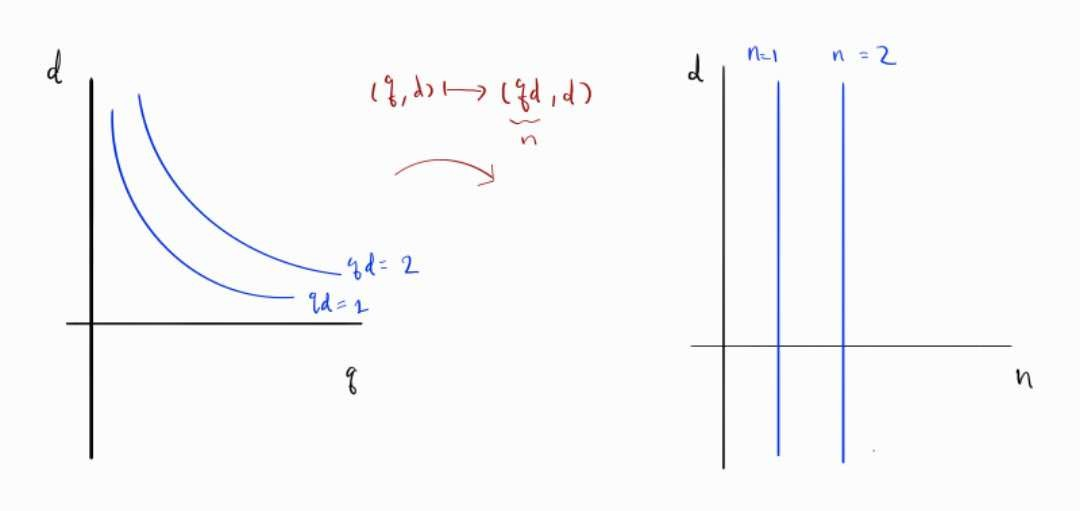
\includegraphics[width=0.8\textwidth]{cover/hyperbola.jpg}
    \caption{example \(x =2 \)}
    \label{fig:mylabel}
\end{figure}

the sum on the left is indeed the number of integer points in a family of hyperbolas, it allows us to rewrite the sum of dirichlet convolution as following
\[\sum_{n \leq x}(a*b)(n) = \sum_{n \leq x} \sum_{d | n}a(d)b(n/d) = \sum_{qd \leq x}a(d)b(q) = \sum_{d \leq x}a(d)\sum_{q \leq x/d}b(q)\]


\begin{colorexample}(Dirichlet's formula) For any \(x\geq 1\), we have
    \[\sum_{n \leq x} \tau(n) = x \log x + (2C-1)x +O(x^{1/2})\]
    where \(C\) is the euler constant, and a rougher estimate is 
    \[\sum_{n \leq x} \tau(n) = x \log x + O(x)\]
\end{colorexample}

\begin{proof}
    By hyberbola method \(\sum_{n \leq x} \tau(n) = \sum_{d \leq x} \sum_{q \leq x/d} 1 = \sum_{d \leq x} [\frac{x}{d}]\),
    so if we estimate \([\frac{x}{d}] \leq \frac{x}{d}\) and apply the asymptotic formula for harmonic series we can get a rough estimate. To get a refined estimate, we reconsider \(\sum_{n \leq x} \tau(x) = \sum_{qd \leq x} 1\) to count the lattice, notice that the number of lattice on the line \(q = d\) are \([\sqrt{x}]\), and the distribution of lattice are symmetric with respect to the line, so we have
    \begin{align*}
        \sum_{n \leq x} \tau(n) &= (2 \sum_{qd \leq x, d \leq \sqrt{x}}1) - [\sqrt{x}]^2 \\
        &= (2 \sum_{d \leq \sqrt{x}} [\frac{x}{d}]) - [\sqrt{x}]^2  \\
        &= \{2 \sum_{d \leq \sqrt{x}} \frac{x}{d} + O(1)\} - \{\sqrt{x}+O(1)\}^2 \\
        &= \{2x \sum_{d \leq \sqrt{x}} \frac{1}{d} \} + O([\sqrt{x}]) - \{x + O(\sqrt{x})\} \\
        &= 2x\{\log \sqrt{x} + C + O(1/\sqrt{x})\} - x + O(\sqrt{x}) \\
        &= x \log x + (2C-1)x + O(\sqrt{x})
    \end{align*}
\end{proof} 



\subsubsection{periodic arithmetic function}

\begin{definition}
    An arithmetic function \(f: \nn \to \cc\) is called periodic if there exists a positive integer \(k\) such that
    \[f(n+k) = f(n)\]
    for all \(n \in \nn\), and we call the smallest such \(k\) the (fundamental) period of \(f\).
\end{definition}

\begin{remark}
    \textbf{The fundamental period is unique}, and it divides any other period of \(f\). In fact, if we set \(\mathcal{P}\) as the set of all periods of \(f\), as a non-empty subset of \(\nn\), it has a minimum element \(k\). If \(N\) is another period, by the division we have \(N = qk+ r\) for some \(q \in \nn\) and \(0 \leq r < k\), hence we have
    \[f(n) = f(n+N) = f(n+r+qk) = f(n+r)\]
    for any \(n \in \nn\), hence \(r\) is also a period of \(f\) if \(r \neq 0\), hence \(\mathcal{P} = k\nn^*\) exactly.
\end{remark}

\begin{colorexample}
    A natural example is exponential function, for the sake of notation,
    \[e(n) = e^{2\pi i n}\]
    it is a 1-peridoic function.
\end{colorexample}

\begin{theorem}[finite Fourier series] $ \\$ \label{ffs}
    Let \(f\) be an arithmetical function with period \(k\), then there exists a unique arithmetical function \(\hat{f}\) such that 
    \[f(m ) = \sum_{n = 1}^k\hat{f}(n) e(\frac{mn}{k})\]
    In fact \(\hat{f}\) is the fourier transform of \(f\) on \(\zz/k\zz\) by
    \[\hat{f}(n) = \frac{1}{k}\sum_{m = 1}^k f(m) e(-\frac{mn}{k})\]
    
\end{theorem}

\subsection{Character}

\begin{definition}
    Let \(G\) be a finite abelian group, a \textbf{character} of \(G\) is a group homomorphism \(\chi : G \to \cc^\times\), and we denote the set of all characters of \(G\) as \(\hat{G}\), it forms a group under function multiplication
    \[\forall g \in G: (\chi_1\cdot \chi_2)(g) : = \chi_1(g)\chi_2(g)\]
    And we call \(\hat{G}\) the \textbf{Character group} of \(G\).
\end{definition}

Here are some quick obeservations:
\begin{itemize}
        \item \textbf{image of character should be in \(\sph^1\)}: any elements \(a \in G\) is of finite order, and homomorphism of groups makes \(\chi(e) = 1\), hence \(\chi(a)^n = 1\) with \(n = ord(a)\).
    \item \textbf{Inverse of character is the complex conjugate}: \(|\chi(n)| = 1\), which allows us to define the inverse
    \[\chi^{-1}(n) = 1/\chi(n) = \bar{\chi}(n)\]
    \item In particular, \(\chi(-1) = \pm 1\) since \(\chi(-1)^2 = \chi(1) = 1\), which allows us to classify the character into two types: \textbf{even} character with \(\chi(-1) = 1\) and \textbf{odd} character with \(\chi(-1) = -1\).
\end{itemize}
\begin{remark}
    We consider the categroy of all abelian groups, denoted by \(\mathbf{Ab}\), the character group can be generalized in the category by a contravariant functor \(\hat{(-)}: \mathbf{Ab} \to \mathbf{Ab}^{op}\): For the object \(G \in \mathbf{Ab}\), we have \(\hat{G} = \Hom(G, \cc^\times)\) ; For the morphism \(f:G \to H\), it induces a morphism between dual groups \(\hat{f}: \hat{H} \to \hat{G}\) by \(\chi \mapsto \chi \circ f\), i.e.
    % https://q.uiver.app/#q=WzAsNCxbMCwwLCJHIl0sWzIsMF0sWzEsMCwiSCJdLFsxLDEsIlxcbWF0aGJie0N9XioiXSxbMiwzLCJcXGNoaSJdLFswLDIsImYiXSxbMCwzLCJcXGhhdHtmfShcXGNoaSkiLDIseyJzdHlsZSI6eyJib2R5Ijp7Im5hbWUiOiJkYXNoZWQifX19XV0=
\[\begin{tikzcd}
	G & H & {} \\
	& {\mathbb{C}^*}
	\arrow["f", from=1-1, to=1-2]
	\arrow["{\hat{f}(\chi)}"', dashed, from=1-1, to=2-2]
	\arrow["\chi", from=1-2, to=2-2]
\end{tikzcd}\]
    However, the functor is not an equivalent since it is not full, that is the reason why we only consider the character group of finite abelian groups.
\end{remark}

\begin{remark}
    Another view of character is that the character is naturally \textbf{a one-dimensional complex representation} of \(G\) since \(\cc^* \cong \GL_1(\cc)\), and any character as such is irreducible.
\end{remark}


\begin{proposition}
    For any finite abelian group \(G\), we have \(\hat{G} \cong G\)
\end{proposition}

\begin{proof}
    For any finite abelian group \(G\), there exists a decomposition of cyclic groups \(G \cong \zz/n_1 \oplus \cdots \oplus \zz/n_r\), the universal property of direct sum allows \(\widehat{G \oplus H} \cong \widehat{G} \times \widehat{H}\) hence we have
    \[\hat{G} \cong \widehat{\zz/n_1}\oplus \cdots \oplus \widehat{\zz/n_{r}}\]
    hence it is enough to prove the isomorphism for any cyclic group \(\zz/n\).
\end{proof}

Here is a useful lemma, which appears in many proofs, from the view of category, it shows that the induced morphism of a injection is a surjection.
\begin{lemma}
    Let \(G\) be a finite abelian group and \(H\) be its subgroup, then for any character \(\chi \in \hat{H}\), there exists exactly \([G:H]\) characters \(\hat{G}\) that extend \(\chi\) to \(G\).
\end{lemma}
\begin{proof}
    Consider restriction map \(r: \hat{G} \to \hat{H}\) defined by \(\chi \mapsto \chi|_H\), it is a group homomorphism, and we will show that \(r\) is surjective, then we consider the equivalence relation on \(\hat{G}\) by
    \[\chi_1 \sim \chi_2 \iff \chi_1|_H = \chi_2|_H\]
    the relation gives that the class of \(\chi\) is exactly the set of characters that extend \(\chi\) to \(G\), and the relation is actually same as the relation defined by cosets of \(\bar{H}\), then we can deduce the number by isomorphism of dual groups:
    \[\#[\chi] = [\hat{G}:\hat{H}] = [G:H]\]

    \textbf{Surjective:} We take \(g_1 \notin H\) and construct a subgroup of \(G\) by
    \[G_1 = \langle H,g_1 \rangle = \{g_1^kh \mid k\in \nn, h \in H\}\]
    then we can extend the character \(\chi\) by defining \(\chi_1(g_1^kh) = \chi(h)\), i.e. we set \(\chi_1(g_1) = 1\) and allow \(\chi_1(ab) = \chi_1(a)\chi_1(b)\), then we can verify that \(\chi_1 \in \widehat{H_1}\) and \(\chi_1|_H = \chi\). Similarly we can construct a chain of subgroups by \(G_k = \langle G_{k-1},g_k \rangle\) with some \(g_k \notin G_{k-1}\), so we have
    \[G_0 = H \subsetneq G_1 \subsetneq \dots \subsetneq G_n = G\]
    the chain will stop since \(G\) is finite (or it is finitely generated \(\zz\)-module, so we can use noetherian condition).
\end{proof}
\begin{remark}
    Notice that \(\cc^*\) is a divisible abelian group, then for any short squence of abelian groups
    \[0 \to H \to G \to G/H \to 0\]
    we have a conversion of exact sequence
    \[0 \to \widehat{G/H} \to \hat{G} \to \hat{H} \to 0\]
    we can talk more if we restrict our view on finite abelian groups.
\end{remark}

\begin{theorem}
    Let \(G\) be a finite abelian group, then any quotient group of \(G\) can be seen as a subgroup of \(G\), furthermore we have
    \[G \cong H \oplus G/H\]
\end{theorem}

\begin{proof}
    We set \(H^\perp = \{\chi \in \hat{G} \mid \chi(h) = 1, \forall h \in H\}\) as the complement of \(\hat{H}\) in \(\hat{G}\), it is natural in the sense of \(\zz\)-module, then we can prove that \(H^{\perp} \cong\widehat{G/H}\). Notice that \(H^{\perp}\) is exactly a subgroup of \(\hat{G}\), and \(H^\perp \cap \hat{H} = \{1_H\}\) , so we have a direct sum \[\hat{G} = \hat{H} \oplus H^\perp \cong \hat{H} \oplus \widehat{G/H}\]
    by the isomprhism of dual groups, we can deduce the result. 
\end{proof}

\begin{proposition}[orthogonality]
    Let \(G\) be a finite abelian group,
    \begin{enumerate}
        \item Fix \(\chi \in \bar{G}\), then \[\sum_{g \in G} \chi(g) = \begin{cases}
            |G|  \quad &\chi = 1 \\
            0 \quad &\chi \neq 1
        \end{cases}\]
        \item Fix \(g \in G\), then \[\sum_{\chi \in \hat{G}} \chi(g) = \begin{cases}
            |G|  \quad &g = e \\
            0 \quad &g \neq e
        \end{cases}\]
    \end{enumerate}
    
\end{proposition}

\begin{proof}
    For the first case, if \(\chi = 1\) then it is trivial, otherwise we can take \(h \in G\) such that \(\chi(h) \neq 1\), and the transaltion \(g \mapsto h^{-1}g\) is a bijection of \(G\), so we have
    \[\sum_{g\in G}\chi(g) = \sum_{g \in G}\chi(h)\chi(h^{-1}g) = \chi(h) \sum_{g \in G}\chi(g)\]
    then we can deduce the result. For the second case, we suppose that \(g \neq e\), then there exists a character \(\psi\) such that \(\psi(g) \neq 1\), and the translation \(\chi \mapsto \psi^{-1}\cdot \chi\) is a bijection of \(\hat{G}\), so we have
    \[\sum_{\chi \in \hat{G}} \chi(g) = \psi(g) \sum_{\chi \in \hat{G}} (\psi^{-1}\cdot 
    \chi)(g) = \psi(g) \sum_{\chi \in \hat{G}} \chi(g)\]
    then we can deduce the result.
\end{proof}

\begin{colorcorollary}
    Let \(a,b \in G\), then we have 
    \[\sum_{\chi \in \hat{G}}\chi(a)\overline{\chi(b)} = \begin{cases}
        |G|  \quad &a = b \\
        0 \quad &a \neq b
    \end{cases}
\]
\end{colorcorollary}

\begin{proof}
    
\end{proof}

A special result of orthogonality is about the structure of the character, we set \(\mathbf{FinAb}\) to be the category of finite abelian groups, as we have mentioned before, there exists a contravariant functor inside the categroy, here we set \(D: \mathbf{FinAb} \to \mathbf{FinAb}^{op}\), the following result shows that the functor is actually an equivalence with \(D^2 = Id\).

\begin{colortheorem}
    Let \(G\) be a finite abelian group, there exists a natural isomorphism \(\phi: G \to \hat{\hat{G}}\) defined by \(g \mapsto \phi_g\) with \(\phi_g(\chi) = \chi(g) \).
\end{colortheorem}
\begin{proof}
    It is easy to verify that the map is a morphism, so it is enough to show injection since it is finite, and we consider the kernel.
    \begin{align*}
        g \in \ker \phi &\iff \phi_g(\chi) = 1, \forall \chi \in \hat{G} \\
        &\iff \chi(g) = 1, \forall \chi \in \hat{G} \\
        &\iff \sum_{\chi \in \hat{G}} \chi(g) = |\hat{G}| = |G| \\
        &\iff g = e
    \end{align*}
\end{proof}

\begin{remark}
    Notice that the map is <<natrual>> since it does not depend on the choice of groups, and we can verify the following diagram commutes for any morphism \(f: G \to H\)
    \[
\begin{tikzcd}
G \arrow[r,"\phi_G"] \arrow[d,"f"'] & \widehat{\widehat{G}} \arrow[d,"D^2(f)"] \\
H \arrow[r,"\phi_H"] & \widehat{\widehat{H}}
\end{tikzcd}
\]
    which ensures that the functor \(D\) is an equivalence, it is a special case of the \textbf{Pontryagin duality} for locally compact abelian groups, since every finite group can be endowed with the discrete topology.
\end{remark}






\subsubsection{Dirichlet Character and Gauss sum}

\begin{definition}
    Let \(N \in \nn^*\), a \textbf{Dirichlet character} modulo \(N\) is a character of the multuplicative group \((\zz/N\zz)^\times\), i.e. \
\[\chi: (\zz/N\zz)^\times \to \cc^\times\]
\end{definition}

Here are some quick descriptions of this type of character: 
\begin{itemize}

    \item Let \(\chi\) be a Dirichlet character modulo \(N\), then we can extend \(\chi\) to a function on \(\zz\) by \[\tilde{\chi}(a) = \begin{cases}
        \chi(\bar{a}) \quad &\gcd(a,N) = 1 \\
        0 \quad &\gcd(a,N) \neq 1
    \end{cases}\]
    It defines an arithmetic function that is \textbf{completely multiplicative} and \textbf{\(N\)-periodic}. Each character can be extended like that, so we sometimes do not distinguish the character and the arithemetic function.
    
    \item The order of \((\zz/N\zz)^\times\) is \(\varphi(N)\) with \(\varphi\) the Euler totient function, so the orthogonality of characters can be written as
    \[\sum_{\chi \in \widehat{(\zz/N\zz)^*}}\chi(a)\overline{\chi(b)} = \begin{cases}
    \varphi(N)  \quad &a \equiv b \mod N \\
    0 \quad &a \not\equiv b \mod N
    \end{cases} \]
    for any \(a,b \in \zz\) with \((b,N) = 1\).

    \item We call a dirchlet character to be \textbf{principal or trival} if \(\chi(g) = 1\) for any \(g \in (\zz/N\zz)^\times\), and we denote the principal character by \(\chi_0\).
\end{itemize}


\begin{theorem}
    Let \(f: \nn \to \cc\) be an arithemetic function is a Dirichlet character modulo \(N\) if it satisfies the following conditions:
    \begin{enumerate} [(a)]
        \item completely multiplicative
        \item \(N\)-periodic for some \(N \in \nn^*\)
        \item \(|f(n)| = 1\) if and only if \(\gcd(n,N) = 1\)
    \end{enumerate}
\end{theorem}
\begin{proof}
    
\end{proof}


\begin{example}
    Notice that \((\zz/3\zz)^\times\) is of order \(2\), so there are exactly two characters, it can be given by the following table:
    \[\begin{tabular}{c| c c c c c c}
$n$      &0 &1 &2 \\
\midrule
$\chi_1$ &0 &1 &1 \\
\midrule
$\chi_2$ &0 &1 &-1 \\
\end{tabular}\]
while \((\zz/6\zz)^\times \cong (\zz/2\zz)^\times \times (\zz/3\zz)^\times\) is of order \(2\), so the dirichlet character mod \(6\) can be given by the product of the chracter mod 2 (trival character) and mod 3 (\(\chi_1\) and \(\chi_2\) as above), and we write down the table
\[\begin{tabular}{c|cccccc}
$n$      &0 &1 &2 &3 &4 &5  \\
\midrule
$\psi_1$ &0 &1 &0 &0 &0 &-1 \\
\midrule
$\psi_2$ &0 &1 &0 &0 &0 &1 \\
    
\end{tabular}\]
\end{example}

\begin{example}
    Another example is the character mod 9, there are exactly 6 characters, while in it there are two characters can be written down by character mod 3
    \[\begin{tabular}{c|ccccccccccc}
$n$      &0 &1 &2 &3 &4 &5 &6 &7 &8  \\
\midrule
$\tilde{\chi_1}$ &0 &1 &-1 &0 &1 &-1 &0 &1 &-1 \\
\midrule
$\tilde{\chi_2}$ &0 &1 &-1 &0 &1 &-1 &0 &1 &-1\\
    \end{tabular}\]
    for instane,
    \[\tilde{\chi}_1(n) = (\chi_1 \cdot f_0)(n) = \begin{cases}
\chi_1(n) \quad &\gcd(n,9) = 1 \\
0 \quad &\gcd(n,9) \neq 1
    \end{cases}\]
    where \(f_0\) is the trival character mod 9, it is clearly that \(\tilde{\chi_1}\) is a 9-periodic function and completely multiplicative, and for any \(n\) coprime with 9 (\(9=3^2\) so also coprime with 3), we have \(\tilde{\chi_1}(n) = \chi_1(n) = \pm 1\), hence it is a dirichlet character mod 9, and the same for \(\tilde{\chi_2}\).
\end{example}

The second example shows that for a dirichlet character mod \(N\), if \(N\) is large then it may be determined by a dirichlet charcter mod the factors of \(N\), which induces the following definition.

\begin{lemma}
    Let \(\chi\) be a dirichlet character mod \(N\), and \(d \) a positive divisor of \(N\), then the following statements are equivalant:
    \begin{enumerate} [(a)]
        \item \(\chi\) factors through \((\zz/d\zz)^\times\): there exists a character \(\psi_d\) mod \(d\) such that the following diagram commutes:
        % https://q.uiver.app/#q=WzAsMyxbMCwwLCIoXFxtYXRoYmJ7Wn0vTlxcbWF0aGJie1p9KV5cXHRpbWVzIl0sWzEsMCwiXFxtYXRoYmJ7Q30iXSxbMCwxLCIoXFxtYXRoYmJ7Wn0vZFxcbWF0aGJie1p9KV5cXHRpbWVzIl0sWzAsMSwiXFxjaGkiXSxbMCwyLCJcXHBpIiwyXSxbMiwxLCJcXGNoaV9kIiwyXV0=
\[\begin{tikzcd}
	{(\mathbb{Z}/N\mathbb{Z})^\times} & {\mathbb{C}} \\
	{(\mathbb{Z}/d\mathbb{Z})^\times}
	\arrow["\chi", from=1-1, to=1-2]
	\arrow["\pi"', from=1-1, to=2-1]
	\arrow["{\psi_d}"', from=2-1, to=1-2]
\end{tikzcd}\]
        where \(\pi\) is the natural projection sending \([x]_N\) to \([x]_d\).
        \item \(\chi(a) = 1\) for any \(a \in \nn\) such that \(\gcd(a,N) = 1\) and \(a \equiv 1 \mod d\).
        
        \item there is a character \(\psi_d\) mod \(d\) such that in the sense of arithemetic function
        \[\chi(n) = \psi_d(n)\chi_0(n)\]
    \end{enumerate}
    If one of the above statements holds, we say that \(d\) is an \textbf{induced modulus} of \(\chi\).
\end{lemma}

\begin{proof}
    
\end{proof}

\begin{remark}
    Notice that \(N\) is alaways an induced modulus of \(\chi\), while \(1\) is an induced modulus of \(\chi\) if and only if \(\chi\) is trival. In above example, \(3\) is an induced modulus of \(\tilde{\chi}_1\) and \(\tilde{\chi}_2\).
\end{remark}



\begin{colordefinition}
    Let \(\chi\) be a dirichlet character mod \(N\), the conductor of \(\chi\) is the smallest induced modulus of \(\chi\).\\

    The character \(\chi\) is called \textbf{primitive} if its conductor is exactly \(N\).
\end{colordefinition}

\begin{remark}
    \textcolor{blue}{\textbf{Any non-trival charcter mod a prime number \(p\) is primitive}}, since the divisor of \(p\) is only \(1\) and \(p\), so the conductor can only be \(1\) or \(p\), it is \(p\) since the character is non-trival.
\end{remark}

\begin{remark}
    By lemma, for any dirichlet chracter \(\chi\) mod \(N\), there exists a unique primitive character \(\psi\) mod conductor of \(\chi\), such that 
    \[\chi(n) = \psi(n)\chi_0(n)\]
    the proof depends on the fact that conductor is the smallest induced modulus (cf.~\cite{Apostol}, Theorem 8.18).
\end{remark}

Notice that \textcolor{blue}{ dirichlet character can be viewed as a periodic arithemetic function, which allows us to consider its fourier transform}, here is the notation introduced by Gauss in the study of quadratic reciprocity.

\begin{colordefinition}
    The \textbf{Gauss sum} of a dirichlet character \(\chi\) mod \(N\) is defined by
    \[G(n,\chi) = \sum_{m = 1}^N \chi(m) e(\frac{mn}{N})\]
    and we write \(\tau(\chi) = G(1,\chi)\) for convenience.
\end{colordefinition}



\begin{lemma}
    If \(\chi\) is a dirichlet character mod \(N\), then for any \(\gcd(n,N) = 1\) we have
    \[G(n,\chi) = \bar{\chi}(n)\tau(\chi)\]
\end{lemma}

\begin{proof}
    
\end{proof}


    \(\chi\) can be viewed as a function on \(\zz/N\zz\), so by theorem \ref{ffs} we can rewrite
    \[G(n,\chi) = N \cdot \hat{\chi}(-n) \]
    so we can desrible primitive character by gauss sum again, since we believe that fourier transform can keep the information of the original function.

\begin{lemma}
    Along above notation, the following statements are equivalent:
    \begin{enumerate} [(a)]
    \item \(\chi\) is primitive.
    \item \(G(n,\chi) = \bar{\chi}(n) \tau(\chi)\) for any \(n \in \nn\).
    \item \(G(n,\chi) = 0\) for any \(\gcd(n,N) \neq 1\).
    \end{enumerate}
    If one of the above statements holds, we call the Gauss sum is \textbf{separable}.
\end{lemma}
\begin{proof}
    
\end{proof}

\begin{proposition}
    Let \(\chi\) be a primitive character mod \(N\), then
    \[|G(n,\chi)| = \begin{cases}
        \sqrt{N} \quad &\gcd(n,N) = 1 \\
        0 \quad &\gcd(n,N) \neq 1
    \end{cases}\]
\end{proposition}

\begin{proof}
    
\end{proof}

\begin{remark}
    If \(\chi\) is not primitive, then by Ramanujan sum we can show that 
    \[\tau(\chi) = 0\]
\end{remark}

Finally, when the character is primitive, then the fourier expansion of character will be simple since the guass sum is separable, we can conclude that as following, which is important in many applications.

\begin{colortheorem}
    Let \(\chi\) be a primitive character mod \(N\), then its fourier trnasform is 
    \[\hat{\chi} = \frac{\tau(\chi) \bar{\chi}(-1)}{N} \cdot \bar{\chi}\]
    with the fourier expansion
    \[\chi(n) = \frac{\tau(\chi)}{N} \sum_{m = 1}^N \bar{\chi}(n) e(-\frac{mn}{N})\]
\end{colortheorem}

\begin{proof}
    
\end{proof}

\subsubsection{Legendre Symbol and real character}
A character of a finite abelian group is called \textbf{real character} if its image is contained in \(\{\pm 1\}\), this parts is to introduce a typcial example of real character.

Historically, a classical diophantine problem is to solve
\[X^2 = b \mod p\]
with \(p\) a prime, and \(b\) is a given non-zero intger, equivalently, solve the quadratic equation in the finite field \(\ff_p\). For example,
\(X^2 - 2 = 0\) has no solution in \(\ff_5\) while it has solution in \(\ff_3\).

\begin{lemma}
    Let \(p\) be an odd prime, then \(\varphi: \ff_p^* \to \ff_p^*\) with \(x \mapsto x^{\frac{p-1}{2}}\) defines a homomorphism of groups, with kernel \(S_p\) the set of all squares in \(\ff_p^*\), and the image is \(\{1,-1\}\).
\end{lemma}
\begin{proof}
    \(p\) is prime so \(\frac{p-1}{2}\) is an integer, which is enough to show the map is a homomorphism. Notice that \(S_p \subset \ker \varphi\), it is enough to show that \(|S_P| = |\ker \varphi| = \frac{p-1}{2}\). After that, the cardianlity of the image is \(2\), and \(\varphi(x)\) is exactly the roots of \(X^2-1 = 0\), which implies the image is \(\{1,-1\}\).

    \(S_p\) is the image of morphism \(f(x) = x^2\) inside \(\ff_p^*\), the kernel of \(f\) is exactly the solutions of \(X^2-1=0\) in \(\ff_p\), they are exactly \({-1,1}\) since there are at most two distinct solutions, hence \(|S_p| = |\ff_p^*/\ker f| = \frac{p-1}{2}\).

    \(\varphi(x) = 1\) means that \(x\) is a roots of \(X^{\frac{p-1}{2}} - 1 = 0\) in \(\ff_p\), which has at most \(\frac{p-1}{2}\) distinct solutions, hence \(|\ker \varphi| \leq \frac{p-1}{2} = |S_p|\), so immediately \(\ker \varphi = S_p\).
\end{proof}

\begin{colordefinition}
    A integer \(a\) is called a \textbf{quadratic residue} modulo \(p\) if \(a\) is a square in \(\ff_p\), i.e. the diophantine equation
    \[x^2 \equiv a \mod p\]
    has a solution in \(\ff_p\). The \textbf{legendre symbol} is a function defined by
    \[\legendre{a}{p} = \begin{cases}
        0 & a = 0 \mod p \\
        1 & a \text{ is a non-zero quadratic residue modulo } p \\
        -1 &  \text{ otherwise }
    \end{cases}\]
    where \(p\) is an odd prime and \(a\) is an integer.
\end{colordefinition}

Here are some quick descriptions:

\begin{itemize}
    \item If \(p = 2\), then any elements in \(\ff_2\) is square, so legndre symbol makes no sense to distinguish the quadratic residue, hence we only consider odd prime \(p\).

    \item If we fixed the prime \(p\), then the legendre symbol is a extension of the character on \((\zz/p\zz)^\times\) defined by \(a \mapsto a^{\frac{p-1}{2}}\) in the above lemma, exactly it is \textbf{a real primitive character mod \(p\)}.
    
    \item \textcolor{blue}{It is the unique non-trival real character mod \(p\):} In fact, \((\zz/p\zz)^\times\) is a cyclic group of order \(p-1\), so we can choose a generator \(g\), then the character will depend only on \(\chi(g) = \{\pm 1\}\), if \(\chi(g) = 1\), then \(\chi\) is trival, hence along the last statement, we can conclude.
\end{itemize} 

\begin{proposition}
    Let \(a\) be a non-zero square free integer and \(m = 4|a|\), then there exists a unique dirichlet character \(\chi_a\) mod \(m\) such that 
    \[\forall \text{ prime } p \nmid m, \quad \chi_a(p) = \legendre{a}{p}\]
    it will be non-trival if \(a \neq 1\).
\end{proposition}

\begin{proposition}
Let \(p\) be an odd prime, then we have the following formula:
\begin{enumerate}[(a)]
    \item Euler's criterion: \(\legendre{n}{p} = n^{\frac{p-1}{2}} \mod p\) for any intger \(n\).
    \item Gauss's lemma: Let \(n\) be an integer coprime with \(p\), and consider the following numbers:
    \[n,2n,3n,\dots, \frac{p-1}{2}n\]
    For any above numbers, there exists a unique number \(1 \leq a_k \leq p-1\) such that \(a_k = kn \mod p\) with \(1 \leq k \leq \frac{p-1}{2}\), then we have
    \[\legendre{n}{p} = (-1)^s\]
    where \(s\) is the number of \(a_k\) that is greater than \(\frac{p}{2}\).
\end{enumerate}

\end{proposition}


Via the lemma, Gauss proved a remarkable result about the legendre symbol, so-called quadratic reciprocity, for sake of a proof, ~\cite{Apostol} Theorem 9.8 sketches as such style. Here we will see legendre symbol as a character, and consider the gauss sum of other type, such that we can get a series of results about characters.

\begin{lemma}
    The \textbf{ quadratic gauss sum} is defined as 
    \[G_n = \sum_{k=1}^n e(\frac{k^2}{n})\]
    then we have
    \[G_n = \frac{1+i^{-m}}{1+i^{-1}}\sqrt{m} = \begin{cases}
        (1+i)\sqrt{m} & m \equiv 0 \mod 4 \\
        \sqrt{m} & m \equiv 1 \mod 4 \\
        0 & m \equiv 2 \mod 4 \\
        i\sqrt{m} & m \equiv 3 \mod 4
    \end{cases}\]
\end{lemma}

\begin{proof}
    
\end{proof}

\begin{lemma}
    The \textbf{generalized gauss sum} is defined as 
    \[G_n(a) = \sum_{k=1}^n e(\frac{ak^2}{n})\]
    with \(G_n(1) = G_n\) exactly, then we conclude following properties:
    \begin{enumerate}[(a)]
        \item If \(\gcd(a,n) = d\), then \(G_n(a) = d \cdot G_{n/d}(a/d)\).
        \begin{center}
            \textcolor{blue}{hence we usually consider the case \(a\) coprime with \(n\)}
        \end{center}

        \item If \(a\) is coprime with \(n = n_1n_2\) and \(n_1\) is corpime with \(n_2\), then 
        \[G_n(a) = G_{n_1}(an_2) G_{n_2}(an_1)\] 

        \item If \(n\) is fixed, then \(a \mapsto G_n(a)\) is \(n\)-periodic and in particular if \(n = p\) is an odd prime then
        \[G_p(a) = \legendre{a}{p} G_p = \legendre{a}{p} \varepsilon_p \sqrt{p}\]
        with a factor depening on \(p\)
        \[\varepsilon_p = \begin{cases}
            1 & p \equiv 1 \mod 4 \\
            i & p \equiv 3 \mod 4
        \end{cases}\]

        \item Let \(p\) be an odd prime, then the gauss sum of legendre symbol \(\chi_p = \legendre{\cdot}{p}\) is exactly \(G_p\) with
        \[\varepsilon(\chi_p) = \varepsilon_p \sqrt{p}\]
    \end{enumerate}
\end{lemma}

\begin{colortheorem}[Quadratic reciprocity]
    Let \(p\) and \(q\) be two distinct odd primes, then we have
    \[\legendre{p}{q} \legendre{q}{p} = (-1)^{\frac{p-1}{2}\cdot \frac{q-1}{2}}\]
\end{colortheorem}
\begin{proof}
    
\end{proof}

\begin{colortheorem}[Gauss sum]
    Let \(n\) be a square-free odd, and \(\chi\) be a real primitive character mod \(n\), then 
    \[\tau(\chi) = \varepsilon_m \sqrt{m}\]
    with
    \[\varepsilon_m = \begin{cases}
        1 & m \equiv 1 \mod 4 \\
        i & m \equiv 3 \mod 4
    \end{cases}\]
\end{colortheorem}
\begin{proof}
    
\end{proof}

\subsection{Riemann Zeta-function}

\subsubsection{Analytical Continuation: different methods}

As a core object in number theory, Riemann defines the zeta-function in his short paper \cite{Riemann} as following
\[\zeta(s) = \sum_{n \geq 1}\frac{1}{n^s}\]
The basic description can be given as following:
\begin{enumerate}
    \item \(\zeta\) defines a homomorphic function on the half-plane \(\Re(s) >1\), the reason is that the series is uniformly convergent on any compact subset of the half-plane, and \(s \mapsto n^s\) is a entire function.
    
    \item On the half-plane \(\Re(s) > 1\), we have the Euler product expansion
    \[\zeta(s) = \prod_{p \text{ prime}} \frac{1}{1 - p^{-s}}\]
    which encodes the information of prime numbers into this function, that is the reason why it plays an important role in number theory.

    \item On the half-plane \(\Re(s) > 0\), make use of the Gamma function we have the formula
    \[\frac{\Gamma(1+s)}{n^s} = \int_{0}^{\infty} e^{-nt}\, t^{s} \, \frac{dt}{t}\]
    then some calculation can be done to arrange the formula in the form of Mellin transform:
    \begin{equation} \label{integralrepofzeta}
        \pi^{-s/2} \Gamma(s/2) \zeta(s) =  \int_0^\infty \frac{\Theta(t) -1}{2} \, t^{s/2-1} \, \frac{dt}{t}
    \end{equation}
    with theta function defined by
    \[\Theta(t) := \sum_{n \in \zz}e^{-\pi n^2 t} \quad t>0 \]
    and by the poisson's formula it satisfies the functional equation 
    \begin{equation} \label{fctequationoftheta}
    \Theta(t) = t^{-1/2}\Theta(1/t)
    \end{equation}
\end{enumerate}

It can be proved in half plane by complex analysis with no diffcult, and the analytic continuation can be done by mellin transform, the result will be important in number theory, and we state as following:

\begin{colortheorem} \label{completedzetafct}
    Define \(Z(s) = \pi^{-s/2} \Gamma(s/2) \zeta(s)\) as the c\textbf{ompleted zeta-function}, then \(Z\) is holomorphic on half plane \(\Re(s) >1\) and it satisfies
    \begin{enumerate}
        \item \(Z\) has an meomorphic continuation the whole complex plane.
        \item \(Z\) has the only simple poles at \(s = 0\) and \(s = 1\) with residue \(-1\) and \(1\) respectively.
        \item For any \(s \neq 0,1\), functional equation is \(Z(1-s) = Z(s)\).
    \end{enumerate}
\end{colortheorem}
\begin{proof}
    Set the auxiliary function \(\psi(t) = \frac{\Theta(t) - 1}{2}\) and by equation (\ref{fctequationoftheta}) we have
    \[t^{1/2}(2\psi(t)+1) = 2\psi(1/t)+1, \quad t>0\]
    then we can rewrite the integral representation (\ref{integralrepofzeta}) 
    \begin{align*}
        Z(s) &=  \int_0^{1} \psi(t) t^{\frac{s}{2}-1} dt +  \int_1^{\infty} \psi(t) t^{\frac{s}{2}-1} dt \\
        &=  \int_1^{\infty} \psi(1/t) t^{-s/2} \, \frac{dt}{t} +  \int_1^{\infty} \psi(t) t^{\frac{s}{2}} \, \frac{dt}{t}
    \end{align*}
    plug the reflection fomrula of \(\psi\) into the first integral, we can calculate as following
    \begin{align*}
        Z(s) &=  \frac{1}{2}\int_1^{\infty}t^{-s/2-1/2} dt - \frac{1}{2}\int_1^{\infty} t^{s/2 -1} dt + \int_1^{\infty} \psi(t) (t^{s/2 -1} + t^{-s/2 -1/2}) dt \\
        &= \frac{1}{s-1} - \frac{1}{s} + \int_1^{\infty} \psi(t) (t^{\frac{s}{2}}+ t^{\frac{1-s}{2}}) \, \frac{dt}{t} \\
        &= \frac{1}{s-1} - \frac{1}{s} + F(s) + F(1-s)
    \end{align*}
    with \(F(s) = \int_0^{\infty} \psi(t) t^{s/2} \, dt\), the integrand can be proved to be a entire function since \(\psi\) is rapidly decreasing, so it finishes the proof by a quick verification.
\end{proof}

The consequence is immediately about the zeta function, and such a method can be seen as a standard model to get the analytic continuation and functional equation of L-fuctions.

\begin{colorcorollary}
    Riemann zeta function \(\zeta\) has an analytic continuation to the whole complex plane with only a simple pole at \(s = 1\) with residue \(1\), and it satisfies the functional equation
     \[\zeta(1-s) = 2(2\pi)^{-s} \cos(\frac{\pi s}{2}) \, \Gamma(s) \, \zeta(s) 
    \qquad  s\neq 1,0,-1,-2,\dots\]
\end{colorcorollary}

\begin{proof}
    By completed zeta function, the function
    \[s \mapsto \frac{Z(s)}{\pi^{-\frac{s}{2}} \Gamma\left(\frac{s}{2}\right)}\]
    defines an meomorphic function on the hole complex plane, which concides with \(\zeta\) on the half-plane \(\Re(s)>1\), so it is the analytic continuation of \(\zeta\). Notice that \(\Gamma\) has a simple pole at \(s = 0\), which cancels the simple pole of \(Z\) at \(s = 0\), hence \(\zeta\) is actually holomorphic at \(s = 1\) with residue
    \[\mathrm{Res}_{z=1} \zeta = \lim_{s \to 1}  \frac{(s-1)Z(s)}{\pi^{-s/2} \Gamma(s/2)} = \frac{1}{\pi^{-1/2} \pi^{1/2}} = 1\]
    and the funnctional equation can be derived via the formula of gamma function.
\end{proof}

\subsubsection{The values on \(\zz\) and critical strip}

We rewrite the functional equation of zeta function here
\begin{equation} \label{fcteqofzeta}
    \zeta(1-s) = 2(2\pi)^{-s} \cos(\frac{\pi s}{2}) \, \Gamma(s) \, \zeta(s) 
    \qquad  s\neq 1,0,-1,-2,\dots
\end{equation}
it gives a symmetry of values, and determine when the values is zero.

\begin{example}
    We set \(s= 2\) in the functional equation, then we have
    \[\zeta(-1) = - \frac{1}{2\pi^2} \Gamma(2) \zeta(2) = -1/12\]
    since \(\zeta(2) = -\pi^2/6\) and \(\Gamma(2) = 1\). In another case, we hope the cosine term vanish, for example we set \(s = 3\) then \(\zeta(-2) = 0\), it gives a zero of zeta function.
\end{example}

Following the example, the functional equation (\ref{fcteqofzeta}) establishes a non-vanish relation between the negative odd integers and the positive even integers, to know them all we should firstly know one sides of them. To do that, a remarkable constant is introduced.

\begin{colordefinition}
    The function $z \mapsto \frac{z}{e^z-1}$ is holomorphic near the zeros, with the expansion of the series:
    \[\frac{z}{e^z-1}  = \sum_{n \geq 0 } \frac{B_n}{n!}z^n\]
    the \(n\)-th \textbf{Bernoulli's number} is defined  as $B_n$, with respect to the coefficient of the series. 
\end{colordefinition}

The original definition of Bernoulli's number is given by Jacob Bernoulli in his book "Ars Conjectandi" (1713), he defined the number by the summation of powers:
\[\sum_{k=1}^m k^n = \frac{1}{n+1} \sum_{j=0}^n \binom{n+1}{j} B_j \cdot m^{n+1-j}\]
for any $n,m \in \nn$, and the two definitions can be shown to be equivalent by the method of \textbf{generating function}. The definition of power series is easy for us to calculate the values of Bernoulli's number, for Example
\[B_0 = 1, \quad B_1 = \frac{-1}{2}, \quad B_2 = \frac{1}{6}, \quad B_3 = 0, \quad B_4 = \frac{-1}{30} \quad \dots\]
\begin{lemma}
    The Bernoulli's number is rational, and \(B_{2k+3} = 0\) for any \(k \in \nn\).
\end{lemma}
\begin{proof}
    Obeserve that 
    \[\frac{ze^z}{e^z - 1} = \frac{-z}{e^{-z}-1} \]
    which allows us to write
    \[z = \frac{ze^z}{e^z-1}-\frac{z}{e^z-1} = \sum_{n\geq 0} ((-1)^n-1)\frac{B_n}{n!} \cdot z^n \]
    at the voisinage of zero, hence by comparing the coefficients we can conclude that \(B_0 = 1\) and \(B_n = 0\) for any odd integer \(n \geq 3\). To prove the rationalty, by the properties of analytical function we know
    \[B_n = n! \frac{d^n}{dz^n} \left(\frac{z}{e^z-1}\right) \bigg|_{z=0}\]
    the derivatives can be proved to be a rational number by induction on \(n\), hence the result holds true. 
\end{proof}

\begin{colorproposition}
    Let \(k\) be a positive integer, then \(\zeta(-2k) = 0\) and
    \[\zeta(-n) = - \frac{B_{n+1}}{n+1} \]
    by the functional equation a corollary is that
    \[\zeta(2k) = (-1)^{k+1} \frac{(2\pi)^{2k}B_{2k}}{2(2k)!}  \]
\end{colorproposition}

\begin{proof}
    The first result is immediate by the functional equation (\ref{fcteqofzeta}) by setting \(s = 1+2k\), then \(\Gamma(s)\) and \(\zeta(s)\) are both finite, while the consine term vanishes, hence \(\zeta(-2k) = 0\). 
    
    For the second result, a classical formula about cotangent function is
    \[\pi z \cot(\pi z) = 1 + \sum_{n=1}^\infty \frac{2z^2}{z^2 - n^2}, \qquad z \in \cc \backslash  \zz\]
    and we can expand the formula by geometric series as following
    \begin{align*}
        \pi z \cot(\pi z) &= 1 + 2z^2 \sum_{n\geq 1} \frac{-1}{n^2} \cdot \frac{1}{1 - z^2/n^2} \\
        &= 1 - 2z^2 \sum_{n\geq 1} \frac{1}{n^2} \sum_{k\geq 0} \left(\frac{z^2}{n^2}\right)^k \\
        &= 1 - 2 \sum_{k \geq 1} \zeta(2k) z^{2k}
    \end{align*}
    here the formula holds true for $|z|<1$, and the last equality holds by Fubini's theorem, so we get a power series expansion at zeros. To finish the proof, we write the trigonometric function in terms of exponential function, then we can calculate
    \[z \cot(z) = \frac{2iz}{e^{2iz} - 1} + iz = 1+ \sum_{k \geq 1} (-1)^k \frac{2^{2k}}{(2k)!}B_{2k} \cdot z^{2k}\]
    which allows us to get another power series expansion at zeros, if we replace $z$ by $\pi z$ and compare the two expansions, then we can conclude the first formula.
\end{proof}

\begin{remark}
    The absance of values on positive odd integers is a mystery, if we set \(s = 1+2k\) then \(\cos(\pi s/2)= 0\), which prevents us to get any information from the functional equation, although \(\zeta(-2k)\) and \(\zeta(2k+1)\) are lie on two sides, before the work of Apéry in 1978, we even can not determine whether \(\zeta(3)\) is rational or not.
\end{remark}

\begin{remark}
    Another obeservation about zeros is via the completed zeta function
    \[Z(s) = \pi^{-s/2} \Gamma(s/2) \zeta(s)\]
    as we know in theorem \ref{completedzetafct}, \(Z\) is finite at \(s = -2n\), while \(s \mapsto \Gamma(s/2)\) has a simple pole at \(s = -2n\), so the unique possible is that \(\zeta\) has a simple zero at \(s= -2n\) to cancel the pole, and we call such zeros from the Gamma factor the \textbf{trivial zeros} of zeta function.
\end{remark}

\begin{colortheorem}
    \(\zeta\) does not vanish on the line \(\mathrm{Re}(s) = 1\).
\end{colortheorem}

\begin{proof}
    
\end{proof}


\subsubsection{Prime number theorem}



\subsection{Dirichlet L-function}

\subsubsection{Analytical continuation}

\begin{definition}
    \textbf{The dirichlet \(L\)-function associated to a dirichlet character \(\chi\) mod \(N\)} is defined by the series
    \[L(s,\chi) = \sum_{n \geq 1} \frac{\chi(n)}{n^s}\]
\end{definition}

about the analytic properties, some quick descriptions are as following:
\begin{enumerate}
    \item \(s \mapsto L(s,\chi)\) defines a holomorphic function on the half-plane \(\Re(s) > 1\), and the Euler product formula holds as well one the half-plane
    \[L(s,\chi) = \prod_{p \text{ prime}} \frac{1}{1 - \chi(p)p^{-s}}\]
    the prove is similar to the case of zeta function.
    
    \item If \(\chi\) is a character with conductor \(q\) of the form \(\chi = \psi_q \cdot \chi_0 \), where \(\chi_0\) is the trival character mod \(N\) and \(\psi_q\) is a primitive character mod \(q\), then we have the factorization
    \[L(s,\chi) = L(s,\psi_q) \prod_{p \mid N} (1 - \psi_q(p)p^{-s})\]
     which allows us to reduce the analytic properties of \(L(s,\chi)\) to the primitive case.

    \item Riemann zeta function can be viewed as a L-function associated to the character mod \(1\), and for any trival character \(\chi_0\) mod \(N\), we have
    \[L(s,\chi_0) = \sum_{n \geq 1, (n,N) =1} \frac{1}{n^s} = \zeta(s) \prod_{p \mid N} (1 - p^{-s})\]
    so \textcolor{blue}{if \(\chi_0\) is trival, then \(L(s,\chi_0)\) has a meomorhic continuation to the whole complex plane with only a simple pole at \(s = 1\) with residue \(\prod_{p \mid N} (1 - p^{-1})\).}
\end{enumerate}

To do the analytical continuation, we start from the integral we use in the Riemann zeta function
\[\pi^{-\frac{s}{2}}\Gamma(\frac{s}{2})\frac{1}{n^s} = \int_{0}^{\infty}e^{-\pi n^2t}t^{\frac{s}{2}-1} dt \qquad \Re(s)>1\]
to make use of the Gauss sum of the character, so it is natural to modify the integral a little bit \textbf{with a asuumption that the character is non trivial and primitive \(\chi\) mod \(q\)}
\begin{equation} \label{integralrepofdirichletL}
    (q/\pi)^{s/2}\Gamma(\frac{s}{2})\frac{\chi(n)}{n^s} = \frac{1}{\sqrt{q}}\int_{0}^{\infty} [\chi(n)e^{-\pi n^2t/p}]t^{\frac{s}{2}-1}dt
\end{equation}

In the case of \(\chi(-1) = 1\), we can sum equation (\ref{integralrepofdirichletL}) over \(n\) to get 
\begin{equation} \label{evnecharacter}
(q/\pi)^{s/2}\Gamma(\frac{s}{2})L(s,\chi) = \frac{1}{2\sqrt{q}}\int_{0}^{\infty} \psi(t,\chi) \, t^{\frac{s}{2}-1} dt
\end{equation}
with 
\[\psi(t,\chi) =  \sum_{n \in \zz}\chi(n)e^{-\pi n^2 t/q}\]

In the case of \(\chi(-1) = -1\), then \(\psi(t,\chi) = 0\) such that representation (\ref{evnecharacter}) will make no sense in this case, so we should modify the equation (\ref{integralrepofdirichletL}) a little bit (introduce a translation \(s \mapsto s+1\)) to get 
\begin{equation*}
    (q/\pi)^{(s+1)/2}\Gamma(\frac{s+1}{2})\frac{\chi(n)}{n^{s}} = \frac{1}{2\sqrt{q}}\int_{0}^{\infty} \psi(t,\chi) \, t^{\frac{s-1}{2}}dt
\end{equation*}
with
\[\psi(t,\chi) = \sum_{n \in \zz }n \chi(n) e^{-\pi n^2 t/q} \]

above discussion can be summarized as following:

\begin{lemma}
    On the half-plane \(\Re(s) > 1\), the integral repsentation of a  L-function \(L(s,\chi)\) associated to a non-trivial primitive character \(\chi\) mod \(q\) is given by
    \[(q/\pi)^{\frac{s+\mathfrak{v}}{2}}\Gamma(\frac{s+\mathfrak{v}}{2})L(s,\chi) = \frac{1}{2\sqrt{q}}\int_0^{\infty} \psi(t,\chi) t^{\frac{s+\mathfrak{v}}{2}-1} dt\]
    with \(\mathfrak{v} = \frac{1-\chi(-1)}{2}\) and auxiliary function 
    \[\psi(t,\chi) = \sum_{n \in \zz}n^{\mathfrak{v}}\chi(n)e^{-\pi n^2 t/q}\]


\end{lemma}

So we should know the functional equation of \(\psi\) firstly.

\begin{lemma}
    Let \(t>0\), then \(\psi\) satisfies the equation
    \[\tau(\bar{\chi})\psi(t,\chi) = (i/t)^{\mathfrak{v}}\sqrt{q/t} \cdot \psi(\bar{\chi},1/t)\]
    where \(\tau(\chi) = G(1,\chi)\) as the Gauss sum of \(\chi\).

\end{lemma}

\begin{proof}
    We consider the \(f(x) = e^{-\pi x^2t}\) for some \(t>0\), and then we can calculate \[\hat{f}(s) = \frac{1}{\sqrt{t}}f(\frac{s}{t}) = \frac{1}{\sqrt{t}}e^{-\pi s^2/t}\]
    hence by poisson's formula we have
    \begin{equation} \label{lfunpoisson}
        \sum_{n \in \zz}e^{-\pi (n+a)^2 t} = \frac{1}{\sqrt{t}} \sum_{n \in \zz}e^{-\pi n^2/t} e^{2\pi i n a}
    \end{equation}
    now we consider \(\chi\) is a arithemetic function on \(\zz\) with period \(q\), then we can write
    \[\chi(n) = \frac{\tau(\chi)}{q}\sum_{m=1}^{q}\bar{\chi}(m)e^{2\pi i mn/q}\]
    by the primitive character \(\overline{\tau(\chi)} = \chi(-1)\tau(\bar{\chi})\), we have
    \[\tau(\bar{\chi}) \chi(n) = \sum_{m=1}^{q}\bar{\chi}(m)e^{2\pi i mn/q}\]
    hence we can calculate
    \begin{align*}
        \tau(\bar{\chi})\psi(t,\chi) &= \sum_{n \in \zz}n^{\mathfrak{v}}\tau(\bar{\chi})\chi(n)e^{-\pi n^2 t/q} \\
        &= \sum_{m=1}^{q} \bar{\chi}(m) \sum_{n \in \zz} n^{\mathfrak{v}} e^{-\pi n^2 t/q}e^{2 \pi i n m/q} \\
    \end{align*}
    when \(\chi(-1) = 1\), i.e. \(\mathfrak{v} = 0\), we can apply the Poisson's formula (\ref{lfunpoisson}) to get 
    \begin{align*}
        \tau(\bar{\chi})\psi(t,\chi) &= \sqrt{q/t} \cdot \sum_{m=1}^{q} \bar{\chi}(m) \cdot \sum_{n \in \zz} e^{-\pi (qn+m)^2/q t} \\
        &= \sqrt{q/t} \cdot \sum_{l \in \zz} \bar{\chi}(l) e^{-\pi l^2/t} \\
        &= \sqrt{q/t} \cdot \psi(\bar{\chi},1/t)
    \end{align*}
    when \(\chi(-1) = -1\), i.e. \(\mathfrak{v} = 1\), we can modify the poisson's formula (\ref{lfunpoisson}) by taking derivative of \(f(x)\), then we have 
    \[it^{3/2}\sum_{n \in \zz}(n+a) e^{-\pi (n+a)^2 t} = \sum_{n \in \zz} n e^{-\pi n^2/t} e^{2\pi i n a}\]
    then apply it we can get
    \begin{align*}
        \tau(\bar{\chi})\psi(t,\chi) &= \sum_{m=1}^{q} \bar{\chi}(m) \cdot i(q/t)^{3/2} \sum_{n \in \zz} (n+\frac{m}{q}) e^{-\pi (qn+m)^2/qt} \\
        &= (i/t)\sqrt{q/t} \cdot \sum_{l \in \zz} l\cdot\bar{\chi}(l) e^{-\pi l^2/t} \\
        &= (i/t)\sqrt{q/t} \cdot \psi(\bar{\chi},1/t)
    \end{align*}
\end{proof}

Finally we can finish the analytical continuation as we do in Riemann zeta function

\begin{colortheorem}
    For any L-function associated to a non-trivial primitive character \(\chi\) mod \(q\), the completed L-function is defined by
    \[\Lambda(s,\chi) = (q/\pi)^{\frac{s+\mathfrak{v}}{2}}\Gamma(\frac{s+\mathfrak{v}}{2})L(s,\chi)\]
    then \(s \mapsto \Lambda(s,\chi)\) has a \textbf{holomorphic continuation} to the whole complex plane, and it satisfies the functional equation
        \[\Lambda(1-s,\bar{\chi}) = \frac{i^{\mathfrak{v}}\sqrt{q}}{\tau(\chi)} \Lambda(s,\chi) \qquad \] 
\end{colortheorem}

\begin{proof}
    when \(\chi(-1)=1\), i.e. \(\mathfrak{v} = 0\), we have
    \begin{align*}
        2\sqrt{q}\Lambda(s,\chi) &= \int_0^{1} \psi(t,\chi) t^{\frac{s}{2}-1} dt + \int_1^{\infty} \psi(t,\chi) t^{\frac{s}{2}-1} dt \\
        &= \int_{1}^{\infty} \psi(1/u,\chi) u^{-\frac{s}{2}-1} du + \int_1^{\infty} \psi(t,\chi) t^{\frac{s}{2}-1} dt \\
        &= \frac{\tau(\chi)}{\sqrt{q}}\int_{1}^{\infty} \psi(u,\bar{\chi}) u^{\frac{-s-1}{2}} du + \int_1^{\infty} \psi(t,\chi) t^{\frac{s}{2}-1} dt \quad (a)
    \end{align*}
    notice that in this case we have \(\overline{\tau(\chi)} = \tau(\bar{\chi})\), so we can write
    \begin{align*}
        2\sqrt{q}\Lambda(s,\chi) &= \frac{\tau(\chi)}{\sqrt{q}}[\int_{1}^{\infty} \psi(u,\bar{\chi}) u^{\frac{-s-1}{2}} du + \frac{\tau(\bar{\chi})}{\sqrt{q}}\int_1^{\infty} \psi(t,\bar{\chi}) t^{\frac{-s-1}{2}-1} dt] \\
        &= \frac{\tau(\chi)}{\sqrt{q}}\cdot 2\sqrt{q}\Lambda(1-s,\bar{\chi})
    \end{align*}
    Finally, when \(\chi(-1)=-1\), i.e. \(\mathfrak{v} = 1\), we have
    \begin{align*}
        2\sqrt{q}\Lambda(s,\chi) &= \int_0^{1} \psi(t,\chi) t^{\frac{s-1}{2}} dt + \int_1^{\infty} \psi(t,\chi) t^{\frac{s-1}{2}} dt \\
        &= \int_{1}^{\infty} \psi(1/u,\chi) u^{-\frac{s+3}{2}} du + \int_1^{\infty} \psi(t,\chi) t^{\frac{s-1}{2}} dt \\
        &= \frac{\tau(\chi)}{i\sqrt{q}}\int_{1}^{\infty} \psi(u,\bar{\chi}) u^{-\frac{s}{2}} du + \int_1^{\infty} \psi(t,\chi) t^{\frac{s-1}{2}} dt \quad (b)
    \end{align*}
    and notice that in this case we have \(\overline{\tau(\chi)} = -\tau(\bar{\chi})\), so we can write
    \begin{align*}
        2\sqrt{q}\Lambda(s,\chi) &= \frac{\tau(\chi)}{i\sqrt{q}}[\int_{1}^{\infty} \psi(u,\bar{\chi}) u^{-\frac{s}{2}} du + \frac{\tau(\bar{\chi})}{i\sqrt{q}}\int_1^{\infty} \psi(t,\bar{\chi}) t^{\frac{s-1}{2}} dt] \\
        &= \frac{\tau(\chi)}{i\sqrt{q}}\cdot 2\sqrt{q}\Lambda(1-s,\bar{\chi})
    \end{align*}
\end{proof}

\begin{remark}
    Notice that in above proof, (a) and (b) shows that the function\(s \mapsto 2\sqrt{q}\Lambda(s,\chi)\) defines an entire function, since the integrand nicely converges uniformly on \((1,\infty)\), so it indicates the holomoprhic continuation of \(\Lambda\).
\end{remark}

\subsubsection{The arithmetic progressions}

%\begin{proposition}
%    For any finite abelian group \(G\), there exists a natural isomorphism \
%    \[\phi: G \to \hat{\hat{G}}, \quad g \mapsto (\chi \mapsto \chi(g))\]
%\end{proposition}

%\begin{proof}
    
%\end{proof}
